\documentclass[11pt]{report}

\usepackage{amsmath}
\usepackage[inlinechap]{settings/fncystyle}

\input{preamble}
\input{macros}
\input{letterfonts}

\usepackage[indent=0pt]{parskip}

\renewcommand{\chaptername}{Capitolo}
\renewcommand{\contentsname}{Indice}

\title{\Huge{\textbf{Appunti Teoria delle Interazioni Fondamentali}}}
\author{Giacomo Galliani, corso dei prof. A. Vicini, M. Zaro}
\date{Anno accademico 2025-2026}

\begin{document}

\maketitle
\newpage% or \cleardoublepage
% \pdfbookmark[<level>]{<title>}{<dest>}
\pdfbookmark[section]{\contentsname}{toc}
\tableofcontents
\pagebreak

\chapter{Il propagatore di Feyman}
\section{Il propagatore del campo scalare}

Lo scopo principale del corso è capire come si possono fare \emph{praticamete} calcoli di ampiezze di transizione. Poiché trattiamo di particelle elementari, ad energie molto alte, il linguaggio adatto è la teoria quantistica dei campi. A differenza però di un corso in qft, qui considereremo solamente dei campi con dirette applicazioni fisiche. \\

Come detto, vogliamo studiare ampiezze di transizione, cioè processi di scattering. Quasi sempre, penseremo allo scattering fra due (o più) particelle nel modo seguente: all'inizio \(t = -\infty\) abbiamo due particelle infinitamente distanti, che non sentono l'effetto di una sull'altra. Successivamente, le particelle entrano nel range dell'interazione: questo è un punto delicato, dove tipicamente non siamo in grado di risolvere le equazioni esattamente. Dovremo quindi ricorrere a tecniche perturbative. D'altra parte, alla fine abbiamo ancora la \emph{teoria libera}, cioè due particelle che all'infinito non si sentono più. \\

Alla luce di questa discussione qualitativa, è chiaro che il calcolo base che dovremo impostare è la probabilità che una particella venga creata in un punto \(x\), e venga misurata (cioè distrutta) in \(y\). \\

L'elemento di matrice rilevante in questo caso, se consideriamo un campo scalare \(\phi\), è dato da 

\begin{align}
    \bra{0}\phi(y)\phi(x)\ket{0}
\end{align}

Poiché si tratta di un campo scalare, possiamo scrivere 

\begin{align}
    \phi(x) = \int \frac{d^3p}{(2\pi)^3}\frac{1}{\sqrt{2E_p}}(e^{-ipx}a_p + e^{ipx}a^\dagger_p)
\end{align}

dobbiamo allora calcolarci 

\begin{align}
    \bra{0}\int \frac{d^3p}{(2\pi)^3}\frac{1}{\sqrt{2E_p}}(e^{-ipy}a_p + e^{ipy}a^\dagger_p)\int \frac{d^3p'}{(2\pi)^3}\frac{1}{\sqrt{2E_{p'}}}(e^{-ipx}a_{p'} + e^{ipx}a^\dagger_{p'})\ket{0}
\end{align}

Nella teoria quantistica, gli \(a_p, a^\dagger_p\) non sono semplici coefficienti di Fourier, ma sono gli operatori di distruzione e costruzione che obbediscono alle relazioni di commutazione 

\begin{align}
    &[a_p, a^\dagger_{p'}] = (2\pi)^3\delta^3(p-p') \\
    &[a_p, a_{p'}] = 0 \\
    &[a^\dagger_p, a^\dagger_{p'}] = 0 
\end{align}

Ricordando poi che vale \(a_p \ket{0} = 0, \, \forall p\), l'unico contributo non nullo all'integrale viene dal prodotto 

\begin{align}
    a_pa^\dagger_{p'} = a^\dagger_{p'}a_p + (2\pi)^3 \delta^3(p-p')
\end{align}

A questo punto, \(a_p\) annichila il vuoto e l'unico pezzo che conta è il commutatore. L'integrale in \(p'\) a questo punto è banale grazie alla delta di Dirac, ed otteniamo 

\begin{align}
    \bra{0}\int \frac{d^3p}{(2\pi)^3}\frac{1}{2E_p}e^{-ip(y-x)}\ket{0}
\end{align}

Questo oggetto può essere scritto in maniera manifestamente covariante. Basta scrivere il fattore \((2E_p)^{-1}\) come il risultato di un integrale per residui: 

\begin{align}
    \bra{0}\int \frac{d^3p}{(2\pi)^3}\frac{dp_0}{2\pi i }\frac{-e^{-ip(y-x)}}{p^2 - m^2} \ket{0}
\end{align}

Per vedere questo, scrivi \(p^2 -m^2 = p_0^2 -\underbrace{(p_2 + m^2)}_{E^2_p} \). Allora, vista come una funzione della variabile complessa \(p_0\) la funzione ha due poli sull'asse reale, dove \(p_0 = \pm E_p\). Ora dobbiamo scegliere il cammino di integrazione. La scelta tipica è nota come \emph{prescrizione di Feymann}, ed è la seguente: prendi l'asse reale, e circonda con semicerchio \emph{inferiore} il primo polo, con un semicerchio \emph{superiore} il secondo polo. Per chiudere il cammino di integrazione, considera il segno di \(x_0-y_0\): se è positivo, allora chiudi il cammino nel semipiano superiore, se è negativo nel semipiano inferiore.  

\begin{center}
    \begin{tikzpicture}

  % Definisci i parametri
  \def\Ep{2}
  \def\eps{0.3}
  \def\R{4}

  % Disegna gli assi
  \draw[->] (-5,0) -- (5,0) node[right] {Re$(p_0)$};
  \draw[->] (0,-2) -- (0,4) node[above] {Im$(p_0)$};

  % Disegna i poli
  \filldraw (\Ep,0) circle (2pt) node[below] {$E_p$};
  \filldraw (-\Ep,0) circle (2pt) node[above] {$-E_p$};

  % Disegna il cammino di integrazione
  \draw[thick, doc] (-4,0) -- (-\Ep-\eps,0);
  \draw[thick, doc] (-\Ep-\eps,0) arc (180:360:\eps);
  \draw[thick, doc] (-\Ep+\eps,0) -- (\Ep-\eps,0);
  \draw[thick, doc] (\Ep-\eps,0) arc (0:180:\eps);
  \draw[thick, doc] (\Ep+\eps,0) -- (4,0);


\end{tikzpicture}
\end{center}




Questa funzione della differenza \(x-y\) è detta \emph{propagatore}, la indichieremo con \(D(x-y)\), ed è la funzione di green dell'equazione di Klein-Gordon. Ciò vuol dire che soddisfa \footnote{Per verificarlo, passa nello spazio di Fourier. Indicando con \(\tilde{D}(p)\) le componenti di Fourier, trovi allora che deve valere \((p^2 - m^2)\tilde{D}(p) = i\). Da questa ottieni un espressione per \(\tilde{D}\), e scrivendo il propagatore come trasformata di Fourier, ritrovi proprio la nostra espressione. }

\begin{align}
    ((\partial^\mu\partial_\mu)_x + m^2)D(y-x) = -i\delta^4 (x-y)
\end{align}

A partire da questo, si definisce il propagatore di Feymann, come 

\begin{align}
    D_F(x-y) = \begin{cases}
        D(y-x), \, \text{se } y_0 > x_0 \\ 
        D(x-y), \, \text{se } y_0 < x_0  
    \end{cases}
\end{align}

Una nota su come definiamo e normalizziamo gli stati. Noi partiamo sempre dallo stato di vuoto, \(\ket{0}\), che è definito come lo stato che viene annichilito dall'operatore di distruzione, ovvero realizza 

\begin{align}
    a_{\vec{k}} \ket{0} = 0, \, \forall \vec{k}
\end{align}

Invece, agendo su questo con gli operatori di creazione, creiamo gli stati delle particelle. Possiamo agire anche più volte ed ottenere stati di più particelle con lo stesso momento: 

\begin{align}
    &\ket{k} = N_1 a^\dagger_{\vec{k}}\ket{0} \\
    &\ket{2k} = N_2 a^\dagger_{\vec{k}}a^\dagger_{\vec{k}}\ket{0}
\end{align}

questi stati sono tra loro ortogonali. Per vederlo, calcoliamo il prodotto scalare: 

\begin{align}
    \Braket{2k | k} &= N_2^*N_1 \bra{0}a_{\vec{k}}a_{\vec{k}}a^\dagger_{\vec{k}}\ket{0} \\
    &= N_2^* N_1 \bra{0}a_{\vec{k}}(1-a^\dagger_{\vec{k}}a_{\vec{k}})\ket{0} \\
    &= N_2^*N_1 \bra{0}a_{\vec{k}} \ket{0} = 0 
\end{align}

Per avere stati ortonormali, dobbiamo imporre la corretta normalizzazione. Ingenuamente, uno potrebbe richiedere 

\begin{align}
    \Braket{\vec{k} | \vec{k}'} = (2\pi)^3\delta(\vec{k}-\vec{k}')
\end{align}

ma questa in realtà \emph{non} è una scelta corretta, perché non è loretnz-invariante. Per trovare un corretto punto di partenza, considera allora 

\begin{align}
    \frac{d^3 k}{2E_p} = d^4k \delta(k^2 - m^2)\theta(k_0)
\end{align}

che si verifica facilmente da destra verso sinistra, integrando rispetto al tempo, usando le proprietà della delta di Dirac. In particolare, la misura a sinistra è uno scalare di Lorentz. D'altra parte, anche \(d^3k \delta(\vec{k})\) è uno scalare, e posso scrivere 

\begin{align}
    d^3k \delta(\vec{k}) = \left(\frac{d^3k}{2E_p}\right)\delta(\vec{k})2E_p
\end{align}

concludiamo che \(\delta(k)(2E_p)\) è uno scalare! scriveremo allora 

\begin{align}
    \ket{k} = \sqrt{2E}a^\dagger_{\vec{k}}\ket{0}
\end{align}

\section{Il propagatore fermionico}

Consideriamo la lagrangiana di Dirac 

\begin{align}
    \mathcal{L}_{\text{Dirac}} = \bar{\psi}(x)(i\gamma_\mu\partial^\mu -m)\psi(x)
\end{align}

e la conseguente equazione di Dirac, che si ottiene usando le equazioni di eulero-lagrange: 

\begin{align}
    (i\slashed{\partial} -m)\psi(x) =  0, \quad \slashed{\partial} := \gamma_\mu\partial^\mu
\end{align}

La soluzione è scomponibile in onde piane, secondo 

\begin{align}
    \psi(x) = u_{\vec{p}}e^{-ipx} + v_{\vec{p}}e^{ipx}
\end{align}

dove le funzioni \(u, v\) (chiamate spesso \emph{spinori}), obbediscono alle equazioni

\begin{align}
\begin{cases}
    (\slashed{p}-m)u_{\vec{p}} = 0 \\
    (\slashed{p}+m)v_{\vec{p}} = 0 
\end{cases}
\end{align}


la più generale soluzione dell'equazione di Dirac è data da 

\begin{align}
    \psi(x) = \int \frac{d^3p}{\sqrt{2E_{\vec{p}}}(2\pi)^3}\sum_s\left( b^s_{\vec{p}}u^s_{\vec{p}}e^{-ipx} + d^{\dagger, s}_{\vec{p}}v^s_{\vec{p}}e^{ipx} \right)
\end{align}

Ora, quando quantizzo la teoria, voglio che gli stati rispettino la statistica fermionica: questo impone le leggi di \emph{anti-commutazione}: \footnote{c'è un modo semplice di vedere perché questo deve valere. Per la statistica fermionica, è impossibile creare dal vuoto uno stato avente due particelle identiche. Ciò è automaticamente realizzato se valgono le relazioni di anticommutazione, perchè \(b^{\dagger, r}_p b^{\dagger, s}_{p'} \ket{0} = - b^{\dagger, s}_{p'} b^{\dagger, r}_p  \ket{0}\). Dunque gli stati fermionici sono completamente antisimmetrici nelle etichette (momento, spin, ecc.) che li caratterizzano. }

\begin{align}
    \left\{b_{\vec{p}}^r, b_{\vec{p}'}^{\dagger, s}\right\} = (2\pi)^3 \delta_{rs}\delta(\vec{p}-\vec{p}') = \left\{d_{\vec{p}}^r, d_{\vec{p}'}^{\dagger, s}\right\}
\end{align}

Ora che abbiamo chiaro come si descrive un fermione in teoria dei campi, vogliamo calcolare il propagatore fermionico. Questo vuol dire determinare la funzione di green \(S_R(x-y)\), t.c. 

\begin{align}
    (i\slashed{\partial} -m)S_R(x-y) = i\delta(x-y)\mathbb{I}_{4\times 4}
\end{align}

una osservazione importante è che posso allora scrivere \((i\slashed{\partial}+m)D_R(x-y)\), con \(D_R\) il propagatore del campo scalare. Infatti, 

\begin{align}
    (i\slashed{\partial} -m)(i\slashed{\partial} +m)D_R(x-y) = (-\square + m^2)D_R(x-y) = i\delta(x-y)
\end{align}

nell'ultima uguaglianza abbiamo usato il fatto che il propagatore del campo scalare è la funzione di green dell'equazione di Klein-Gordon. Ma allora vale 

\begin{align}
    S_R(x-y) = (i\slashed{\partial} + m)\int \frac{d^4p}{(2\pi)^3}\frac{i}{p^2 -m^2}e^{ip(x-y)} = \int \frac{d^4p}{(2\pi)^3}\frac{i(\slashed{p}+m)}{p^2 -m^2}e^{ip(x-y)} 
\end{align}

d'altra parte, potevamo ottenere immediatamente lo stesso risultato passando in trasformata di Fourier, 

\begin{align}
    i\delta(x-y) = (\slashed{p}-m)S_R(x-y) = \int \frac{d^4p}{(2\pi)^4}(\slashed{p}-m)\tilde{S}_R(p)e^{-ip(x-y)}
\end{align}

Ricordando ora che 

\begin{align}
    i\delta(x-y) = \int \frac{d^4p}{(2\pi)^4}e^{-ip(x-y)}
\end{align}

troviamo dunque che

\begin{align}
    (\slashed{p}-m)\tilde{S}_R = i \implies \tilde{S}_R = \frac{i(\slashed{p}+m)}{p^2-m^2} \implies \tilde{S}_F(p) = \frac{i(\slashed{p}+m)}{p^2 -m^2 +i\eps} 
\end{align}

in accordo con quello precedentemente trovato. 

\section{Il propagatore del fotone}

Cominciamo con lo scrivere la lagrangiana della QED: 

\begin{align}
    \mathcal{L}_{QED} = \bar{\psi}(i \gamma_\mu(\partial^\mu +ieA^\mu) -m)\psi - \frac{1}{4}F_{\mu\nu}F^{\mu\nu} - \mathcal{L}_{GF}
\end{align}

Non tutti i termini sono immediati, dunque spieghiamo lo scopo di ciascun termine: 

\begin{enumerate}
    \item \(F_{\mu\nu}\) è la parte dinamica del campo e.m. Questo permette di ottenere le equazioni di Maxwell \(\partial_\mu F^{\mu\nu} = J^{\nu}\).
    \item Il campo \(A_\mu\) compare anche nel pezzo di lagrangiana di Dirac. Questo termine rappresenta l'accoppiamento fra il potenziale di gauge e i campi di materia. Classicamente, avremmo scritto \(-A_\mu J^\mu\), ma sappiamo che per un fermione di Dirac, la corrente è data da \(J_\mu = -e\bar{\psi}\gamma_\mu \psi\).
    \item Il termine \(\mathcal{L}_{GF}\) è detto gauge fixing. Vedremo più in dettaglio dopo che senza questo termine, la lagrangiana è invariante rispetto a trasformazioni di gauge locali. Questo però genera una ambiguità, che non permette di calcolare il propagatore. Una possibile scelta per il gauge fixing è \(\mathcal{L}_{GF} = -(1/2)(\partial_\mu A^\mu)^2\).  
\end{enumerate}

Vediamo più in dettaglio la trasformazione locale di cui parlavamo. Supponiamo che il campo si trasformi come 

\begin{align}
    \psi(x) \rightarrow \psi'(x) = e^{ie\alpha(x)}\psi(x) \implies \bar{\psi}(x) \rightarrow \bar{\psi}'(x) = \bar{\psi}(x)e^{-ie\alpha(x)}
\end{align}

vediamo come cambia la lagrangiana: la parte di dirac \emph{non} è invariante, infatti 

\begin{align}
    \mathcal{L}_{\text{Dirac}} = \bar{\psi}(i\slashed{\partial} -m)\psi = i \bar{\psi}\slashed{\partial}\psi -m\bar{\psi}\psi
\end{align}

il termine con la massa è invariante, mentre invece il primo termine contiene una derivata che agisce su \(\alpha(x)\), che non è costante per ipotesi. In particolare, calcoliamo

\begin{align}
    \mathcal{L}'_{\text{Dirac}} &= -m\bar{\psi}\psi + i\bar{\psi}e^{-i\alpha(x)}(e^{i\alpha(x)}(\slashed{\partial}\psi) + ie \gamma^\mu \partial_\mu \alpha(x)e^{ie\alpha(x)}\psi) \\
    &= \mathcal{L}_{\text{Dirac}} + i\bar{\psi}(ie\gamma^\mu\partial_\mu)\psi
\end{align}

Dunque, possiamo avere una lagrangiana invariante, se inseriamo un campo che si trasformi come 

\begin{align}
    A_\mu \rightarrow A'_\mu = A_\mu + \partial_\mu\alpha(x)
\end{align}

tipicamente, la lagragiana di Dirac con l'aggiunta di questo termine di interazione, che ci accorgiamo a posteriori essere il termine di accoppiamento materia-campo e.m. della lagrangiana di Maxwell classica, si scrive 

\begin{align}
    \mathcal{L} = \bar{\psi}(i\slashed{D} - m)\psi -\frac{1}{4}F_{\mu\nu}F^{\mu\nu}
\end{align}

dove abbiamo introdotto la \emph{derivata covariante}, data da 

\begin{align}
    D^\mu = \partial^\mu + ieA^\mu
\end{align}

In particolare, per tutto quello che abbiamo detto, vale che 

\begin{align}
    \slashed{D}\psi \rightarrow \slashed{D}\psi' = e^{ie\alpha(x)}\slashed{\psi}
\end{align}

così che la lagrangiana è ad occhio invariante. Una teoria di questo tipo si dice teoria di \emph{gauge}, con gruppo di gauge \(G = U(1)\), perché le trasformazioni \(e^{ie\alpha(x)}\) sono mappe dallo spaziotempo al gruppo di Lie \(U(1)\). \\

In questo caso particolare, gli elementi del gruppo sono rappresentati sempre come scalari. Questo è un caso particolare, che deriva dalla semplicità del gruppo di gauge \(U(1)\). Vedremo che ad esempio in cromodinamica, il gruppo di gauge sarà più complicato, e come questo porti a grande differenze fisiche nella teoria.   

Ora, il campo \(A_\mu\) è descritto da un vettore, quindi ha quattro componenti. Mi chiedo se queste componenti sono \emph{fisiche}, ovvero se sono tutte indipendenti fra di loro. Scopriremo che in realtà solamente due sono indipendenti, e in particolare diremo che il fotone è descritto da due gradi di libertà \emph{trasversali}. Vediamo perché: 

Inanzitutto, c'è la libertà di gauge: il campo è invariante se aggiungo il gradiente di qualunque funzione scalare: dunque posso sempre fissare il gauge ponendo una componente uguale a 0. Chiaramente allora la libertà di gauge toglie un grado di libertà al fotone. 

Ora, quando inserisco il termine di gauge fixing, una parte del tensore \(F_{\mu\nu}\) si ricombina con questo, e forma una divergenza totale, che non contribuisce all'azione, e conseguentemente alle equazioni del moto: si trova che alla fine queste sono date da 

\begin{align}
    \square A^\nu = J^\nu \implies \square \partial_\nu A^\nu = \partial_\nu J^\nu = 0
\end{align}

dove nell'ultima abbiamo usato che \(J^\nu\) è la corrente conservata, associata alle trasformazioni di fase globali. Ma questo significa che se definisco un campo \(\phi\) come 

\begin{align}
    \phi := \partial_\mu A^\mu \implies \square\phi = 0
\end{align}

questo fissa un altro grado di libertà, e dunque gli unici gradi sono 2. Ora, abbiamo accenato al fatto che il gauge fixing serva al calcolo della funzione di green. Vediamo più in dettaglio: il propagatore del fotone è la funzione di Green, cioè la soluzione dell'equazione 

\begin{align}
    \square \triangle^{\mu\nu} - \partial^\mu\partial_\lambda \triangle^{\lambda\nu} = -g^{\mu\nu}\delta(x-y)
\end{align}

questo \emph{senza} il gauge fixing: abbiamo già detto che se introduciamo il secondo termine, allora bisogna semplicemente risolvere 

\begin{align}
    \square \triangle^{\mu\nu} = -g^{\mu\nu}\delta(x-y)
\end{align}

Per risolverla, passiamo nello spazio di Fourier: 

\begin{align}
    \triangle^{\mu\nu} = g^{\mu\nu}\int \frac{d^3 p}{(2\pi)^3}\tilde{\triangle}(p)e^{-ipx} \implies \tilde{\triangle}(p) = p^{-2}
\end{align}

dunque il propagatore del fotone è dato da 

\begin{align}
    \triangle^{\mu\nu} = g^{\mu\nu}\int \frac{d^3p}{(2\pi)^3}\frac{e^{-ipx}}{p^2 +i\eps}
\end{align}

abbiamo menzionato che i due gradi di libertà indipendenti del fotone sono gradi trasversali. Vediamo perché: decomponiamo il campo \(A^\mu\) in termini di Fourier: 

\begin{align}
    A_\mu = \int \frac{d^3k}{\sqrt{2\omega}(2\pi)^3}\sum_s (\eps_\mu^s a_{\vec{k}}^s e^{-ikx} + \eps_\mu^{* , s}a_{\vec{k}}^{\dagger, s}e^{ikx})
\end{align}

ora, i vettori \(\eps_\mu\) che indicano la direzione del fotone, sono vettori quadridimensionali, e come tali posso decomporlo in  

\begin{align}
    \eps_\mu(\vec{k}) = \eps_{T, \mu} + a k_{\mu} + b\bar{k}_\mu
\end{align}

dove in particolare: 

\begin{enumerate}
    \item se scrivo \(k_\mu = (k, \vec{k})\), allora \(\bar{k}_\mu = (k, -\vec{k})\)
    \item Il vettore \(\eps_{T, \mu} = (0, \vec{\eps}_T)\) è un vettore tridimensionale, e \emph{trasversale}: questo vuol dire che soddisfa \(\vec{k}\cdot \vec{\eps}_T = 0\)
\end{enumerate}

Ora, chiaramente poiché se prendo \(\partial_\mu \rightarrow k_\mu\), è chiaro che \(\partial_\mu A^\mu \propto b\). D'altra parte, abbiamo visto che dalle equazioni del moto, \(\partial_\mu A^\mu\) non interagisce con gli altri campi e non partecipa alla dinamica: posso dunque porre \(b=0\). D'altra parte, con una trasformazione di gauge posso sempre porre \(a=0\). Questo prova il nostro punto. 

Questo trova una applicazione pratica nella \emph{somma sulle polarizzazioni}: infatti, spesso vorremo calcolare 

\begin{align}
    \sum_\lambda \eps_\mu(p, \lambda)\eps^\nu (p, \lambda) = \Pi^{\mu\nu}
\end{align}

Ora, qualunque cosa sia \(\Pi^{\mu\nu}\), poiché i vettori di polarizzazione sono trasversali, deve certamente valere che \(\Pi^{\mu\nu}p_\nu = \Pi^{\mu\nu}\bar{p}_\nu = 0\). Non è difficile convincersi che il tensore più generale che soddisfa questa condizione è dato da 

\begin{align}
    \Pi_{\mu\nu} = -g_{\mu\nu} +\frac{p_\mu \bar{p}_\nu + \bar{p}_\mu p_\nu}{p\cdot \bar{p}}
\end{align}

in un calcolo realistico, l'espressione si semplifica ulteriormente. Questo perché se calcolo un elemento di matrice, questo spesso ha la forma 

\begin{align}
    M = M_\mu \eps^\mu_\lambda(p)
\end{align}

D'altra parte, vale l'identità di Ward, che ci dice \(\partial_\mu M^\mu =0 \implies p_\mu M^\mu =0\). Dunque quando prendo il prodotto del tensore \(\Pi^{\mu\nu}\) e lo contraggo con l'elemento di matrice \(\eps_\mu\), solo la parte proporzionale alla metrica sopravvive. Per questo motivo, in tutti i calcoli pratici useremo 

\begin{align}
    \Pi^{\mu\nu} = -g^{\mu\nu}
\end{align}

\subsection{Un primo esempio di calcolo}

Come primo esempio di calcolo di un processo realistico, consideriamo il caso di un fotone, con polarizzazione \(r\) e momento \(p\), che da origine ad una coppia particella - antiparticella, con momenti \(k_1, k_2\) e spin \(s_1, s_2\). \\

Questo è il famoso (e importante) risultato che una coppia elettrone-positrone può formarsi a partire da un fotone incidente. Il suo diagramma di Feynman è dato da 

\begin{center}
    \begin{tikzpicture}
        \begin{feynman}
            \vertex (a); 
            \vertex [right = of a] (b); 
            \vertex [above right = of b] (c) {\(r_1\)}; 
            \vertex [below right = of b] (d) {\(r_2\)}; 
            \diagram{
                (a) -- [boson, edge label = $\gamma$, momentum' = $p$] (b); 
                (d) -- [fermion] (b) -- [fermion] (c); 
            }; 
        \end{feynman}
    \end{tikzpicture}
\end{center}

Calcolare l'elemento di matrice ci permetterà di scrivere la regola di Feyman per questo vertice. Il problema è il seguente, voglio calcolare 

\begin{align}
    \Braket{k_1, k_2 | p} = \bra{0}\sqrt{2E_1}\sqrt{2E_2}b^{r_1}_{k_1}d^{r_2}_{k_2}\underbrace{\left(-i\int d^4x e \bar{\psi}\gamma_\mu \psi A^\mu\right)}_{\text{Hamiltioniana d'interazione}}a^{\dagger, r}_{p}\sqrt{2\omega}\ket{0}
\end{align}

il prossimo step è di scrivere \(\psi, \bar{\psi}, A^\mu\) in trasformata di Fourier, esplicitando così gli operatori di creazione e distruzione. D'altra parte, faccio la seguiente osservazione: poiché il campo \(A^\mu\) moltiplica l'operatore \(a^{\dagger, r}_{p}\), sapendo le relazioni di commutazione di \(a, a^{\dagger}\), posso commutare i due operatori, e \(a\) annichilisce il vuoto. L'unico contributo non nullo avviene quando il commutatore non è banale, cioè quando viene selezionato \(a_p\). Un ragionamento uguale vale anche per \(b, d\) e si trova che l'elemento di matrice diventa 

\begin{align}
    \Braket{k_1, k_2 | p} = (-ie)\int d^4x \bra{0}\bar{u}^{r_1}_{k_1}e^{ik_1 x}\gamma_\mu v^{r_s}_{k_2}e^{ik_2 x}\eps^{\mu, r}e^{-ipx}\ket{0}
\end{align}

In particolare, gli esponenziali che rimangono dallo sviluppo di Fourier si ricombinano in una delta di Dirac, che esprime la conservazione dell'impulso: 

\begin{align}
    \Braket{k_1, k_2 | p} = (-ie)(2\pi)^4\delta(k_1 + k_2 -p)\bar{u}_{k_1}\gamma^\mu v_{k_2}\eps_{\mu}(p)
\end{align}

notiamo in particolare il coefficiente \(-ie\gamma^\mu\): questo è particolare di questo vertice, ed è la sua regola di Feyman. \\

Oltre alla regola specifica del vertice, osserviamo una proprietà universale di questi processi: per ogni fermione entrante, questo porta con se \(u(p)\), per ogni anti-fermione entrante, questo porta con sè \(\bar{v}(p)\). Similmente, se il fermione è uscente porta \(\bar{u}(p)\), e un antifermione uscente \(v(p)\). Non è difficile convincersi che queste regole discendono dalle relazioni di commutazione degli operatori di creazione e distruzione. 


\chapter{La teoria dell'urto}

Siamo pronti ad applicare quello che abbiamo imparato per cominciare a fare dei conti pratici: vogliamo calcolare degli elementi di matrice, al fine di determinare la sezione d'urto di alcuni processi fisici. \\

Ma cosa è una sezione d'urto? vediamolo con un esempio schematico. Abbiamo un insieme di particelle, di tipo B, che vengono lanciate contro un bersaglio, ovvero delle particelle di tipo A. L'impatto avviene su una superficie \(S\). Se pensiamo che le particelle di tipo B siano in un cubetto di lato \(\ell_B\) e di densità \(\rho_B\), e il bersaglio sia di lato \(\ell_A\) e di densità \(\rho_A\), è intuitivo che varrà

\begin{align}
    N_{\text{eventi}} \propto \rho_A \rho_B \ell_A \ell_B S
\end{align}

La \emph{sezione d'urto} \(\sigma\) è definita come la costante di proporzionalità. Dimensionalmente, è un area. Uno può pensarla come l'area effettiva delle particelle di tipo A, viste dalle particelle di tipo B. \\

Ora, immaginiamo che le particelle di tipo B vengano lanciate sul bersaglio, tutte ad una diversa altezza. Se indichiamo con \(b\) il \emph{parametro d'impatto}, cioè la distanza minima fra la particella e il bersaglio, tutte le particelle B avranno diverso parametro di impatto. Indicata con \(P(b)\) la probabilità che avvenga l'impatto dato un certo parametro di impatto (quantità che tipicamente viene fornita dalla teoria di campo), allora vale 

\begin{align}
    N_{\text{eventi}} = \int d^2b \rho_B \ell_B P(b) = \rho_B \ell_B \int d^2b  P(b) 
\end{align}

Se il bersaglio è singolo, \(N_A = 1\), e \(N_B = \frac{N_B}{S}\sigma = \rho_B \ell_B \sigma \). Concludiamo allora che 

\begin{align}
    \sigma = \int d^2b P(b)
\end{align}

Il calcolo di questo integrale è particolarmente tedioso, perché in \(P(b) = |\Braket{i|f}|^2\) vorremo scrivere gli stati iniziali e finali come autostati dell'impulso. D'altra parte, dobbiamo effettuare l'integrale nello spazio. Dovremmo quindi prendere dei pachetti d'onda piccati, e poi alla fine del conto prendere il limite di pacchetto molto piccato. Alla fine del lungo calcolo, si trova che 

\begin{align}
    d\sigma = dp_f \frac{(2\pi)^4 \delta(P_A + P_B - P_f)M^2_{AB \rightarrow f}}{4E_AE_B |p_{z,A}/E_A + p_{z,B}/E_B|}
\end{align}

Il differenziale \(dp_f\) rappresenta un volumetto infinitesimo nello spazio delle fasi. In generale, per \(n\) corpi nello stato finale si scrive 

\begin{align}
    dp_f = \left(\prod_i^n \frac{d^3p_i}{(2\pi)^3 2E_i} \right)(2\pi)^4 \delta(p_{IN} - \sum_i p_i)
\end{align}

Per fissare meglio le idee, vediamo invece come si scrive per due corpi finali. Allora avremmo 

\begin{align}
    dp_{f2} = \frac{d^3p_1 d^3p_2}{(2\pi)^2 4E_1E_2}\delta(p_1 + p_2 -p_{IN})
\end{align}

Nel caso più gerale, i due corpi hanno masse diverse. Questo vuol dire che \(p_1^2 = m_1^2 \neq p_2^2 = m_2^2\). Posso usare la delta per integrare in \(d^3p_2\), ed ottenere 

\begin{align}
    dp_{f2} = \frac{d^3p_1}{(2\pi)^2 4E_1E_2}\delta(E_1 +E_2 - E_{IN}) = \frac{p_1^2 dp_1 d\Omega^2}{(2\pi)^2 4E_1E_2}\delta(E_1 +E_2 - E_{IN})
\end{align}

Ora, vorremo usare l'ultima delta nell'energia per integrare in \(dp_1\). Per farlo, devo scrivere 

\begin{align}
    \delta(E_1+E_2-E_{IN}) = \delta(p_1 - \bar{p}_1)\left(\frac{d}{dp_1}(E_1 + E_2 -E_{IN}) \right)^{-1}
\end{align}

Per trovare \(\bar{p}_1\) si tratta solamente di algebra, perché possiamo metterci nel SR del centro di massa dove \(P_{IN} = 0\), e scriveremo \(E_{1} = \sqrt{m_1^2 + p_1^2}, \, E_{2} = \sqrt{m_2^2 + p_2^2}, \, E_{IN} = \sqrt{m_1^2 m_2^2 + 2p_1^2}\). Si trova infine che 

\begin{align}
    \bar{p}^2_1 = \frac{E^4_{IN} + m_1^4 + m_2^4 -2E_{IN}^2 m_1^2 -2E^2_{IN}m_2^2 - 2m_1^2m_2^2}{4E^2_{IN}} = \frac{\lambda(E^2_{IN}, m_1^2, m_2^2)}{4E^2_{IN}}
\end{align}

Troviamo infine che vale 

\begin{align}
    dp_{f2} = \frac{d\varphi d\cos\theta}{16\pi^2}\frac{\bar{p}_1}{E_{IN}}
\end{align}

\section{Calcolo del processo \(e^+e^- \rightarrow \mu^+\mu^-\)}

Consideriamo ora la lagrangiana 

\begin{align}
    \mathcal{L} = \underbrace{i\bar{\psi}_e \slashed{D}\psi_e -m_e\bar{\psi}_e\psi_e}_{\text{elettrone}} + \underbrace{i\bar{\psi}_\mu \slashed{D}\psi_\mu -m_\mu\bar{\psi}_\mu\psi_\mu}_{\text{muone}} - \underbrace{\frac{1}{4}F_{\mu\nu}F^{\mu\nu}}_{\text{fotone}} 
\end{align}

Poichè la derivata convariante è la stessa che agisce su entrambi i campi di materia, e ricordando che vale \(D_\mu = \partial_\mu -ieA_\mu\), i due campi hanno diversa massa ma stessa carica (che è proprio quello che succede sperimentalmente con elettrone e muone). 

\nt{Poichè i due campi di materia compaiono disaccopiati, questo vuol dire che i due campi non interagiscono direttamente tra di loro. Ad esempio, un processo del tipo 

    \begin{center}
    \begin{tikzpicture}
        \begin{feynman}
            \vertex (a); 
            \vertex [above left = of a ] (b) {$e^-$}; 
            \vertex [below left = of a] (c) {$\mu^+$}; 
            \vertex [right = of a ] (d) {$\gamma$}; 

            \diagram{
                (b) -- [fermion] (a) -- [fermion] (c); 
                (a) -- [boson] (d); 
            }; 
        \end{feynman}
    \end{tikzpicture}
    \end{center}

    \emph{non} è permesso da questa teoria. (e in effetti non si osserva neanche in natura)
}

Ora, quello che noi faremo è calcolare processi al \emph{primo ordine}. Questo vuol dire che considereremo dei diagrammi ad albero, dove non ci sono dei loop chiusi. In particolare, il primo step è sempre disegnare le particelle uscenti ed entranti: 

\begin{center}
    \begin{tikzpicture}
        \begin{feynman}
            \vertex (a); 
            \vertex [above left = of a ] (b) {$e^-$}; 
            \vertex [below left = of a] (c) {$e^+$}; 
            \vertex [right = of a ] (d);
            \vertex [above right = of d ] (e) {$\mu^-$};
            \vertex [below right = of d ] (f) {$\mu^+$}; 


            \diagram{
                (b) -- [fermion] (a) -- [fermion] (c); 
                %(a) -- [boson] (d); 
                (e) -- [fermion] (d) -- [fermion] (f)
            }; 
        \end{feynman}
    \end{tikzpicture}
\end{center}

A questo punto, bisogna collegare il diagramma in modo che 

\begin{enumerate}
    \item Tutti i processi siano permessi dalla lagrangiana 
    \item Non si formino loop chiusi
\end{enumerate}

In questo caso, l'unica possibilità è data da \footnote{In caso ci fossero più possibilità, dobbiamo considerarle tutte separatamente e sommare su queste}

\begin{center}
    \begin{tikzpicture}
        \begin{feynman}
            \vertex (a); 
            \vertex [above left = of a ] (b) {$e^-$}; 
            \vertex [below left = of a] (c) {$e^+$}; 
            \vertex [right = of a ] (d);
            \vertex [above right = of d ] (e) {$\mu^-$};
            \vertex [below right = of d ] (f) {$\mu^+$}; 


            \diagram{
                (b) -- [fermion] (a) -- [fermion] (c); 
                (a) -- [boson, edge label = $\gamma$] (d); 
                (e) -- [fermion] (d) -- [fermion] (f)
            }; 
        \end{feynman}
    \end{tikzpicture}
\end{center}

Usando le regole di feynman che abbiamo visto, è l'elemento di matrice legato a questo processo sarà dato da 

\begin{align}
    M_{\vec{s}} = \bar{v}_{s_1}(p_1)(ie\gamma_\mu)u_{s_2}(p_2)\frac{-ig^{\mu\nu}}{(p_1 + p_2)^2 +i\eps}\bar{u}_{s_3}(p_3)(ie\gamma_\nu)v_{s_4}(p_4)
\end{align}

Infatti: 

\begin{enumerate}
    \item Nel primo pezzo riconosco il vertice calcolato nella sezione precedente. Questo spiega il fattore \(ie\gamma_\mu\). D'altra parte, ho una particella \(e^-\) entrante con momento \(p_2\), che porta con sé un fattore \(u(p_2)\), mentre il positrone con momento \(p_1\) porta un fattore \(\bar{v}(p_1)\). 
    \item In mezzo, il fotone deve propagarsi: dunque riconosciamo il propagatore del fotone, con momento \(p_1+p_2\), grazie alla conservazione del momento 
    \item I fattori della fine si ottengono esattamente come quelli del primo pezzo. 
\end{enumerate}

Per calcolare la probabilità del processo dobbiamo calcolare 

\begin{align}
    P_{e^+e^- \rightarrow \mu^+\mu^-} = \abs{M_{\vec{s}}}^2 = M_{\vec{s}}M^*_{\vec{s}}
\end{align}

dobbiamo quindi calcolarci \(M^*_{\vec{s}}\). Andiamo per pezzi, abbiamo che: 

\begin{align}
    (\bar{v}(p_1)ie\gamma^\mu u(p_2))^* = (-ie)u^+(p_2)(\gamma^0\gamma^\mu)^+v(p_1)
\end{align}

Ricordando che \(\gamma^{0+} = \gamma^0\), si ha che 

\begin{align}
    (\bar{v}(p_1)ie\gamma^\mu u(p_2))^* = (-ie)u^+(p_2)\gamma^{\mu +}\gamma0 v(p_1)
\end{align}

ora, \(\gamma^{\mu +}\gamma^0 = \gamma^0\gamma^{\mu}\), e quindi 

\begin{align}
    (\bar{v}(p_1)ie\gamma^\mu u(p_2))^* &= (-ie)u^+(p_2)\gamma0\gamma^{\mu} v(p_1) \\
    &= (-ie)\bar{u}(p_2)\gamma^{\mu} v(p_1)
\end{align}


\nt{Prendere il complesso coniugato equivale a percorrere la linea fermionica al contrario!}

L'intero complesso coniugato dell'elemento di matrice sarà allora dato da 

\begin{align}
    M^*_{\vec{s}} = v_{s_1}(p_1)(-ie\gamma_\mu)\bar{u}_{s_2}(p_2)\frac{ig^{\mu\nu}}{(p_1 + p_2)^2 -i\eps}u_{s_3}(p_3)(-ie\gamma_\nu)\bar{v}_{s_4}(p_4)
\end{align}

a \emph{polarizzazione fissata} \(\vec{s} = (s_1, s_2, s_3, s_4)\), la probabilità del processo è data da \(M_{\vec{s}}M^*_{\vec{s}}\). D'altra parte, molte volte, e la cosa semplifica anche i calcoli, noi non misuriamo lo spin di questi oggetti, e possiamo \emph{sommare sulle polarizzazioni}: 

\begin{align}
    P_{e^+e^- \rightarrow \mu^+\mu^-} = \sum_{\vec{s}}(MM^*)_{\vec{s}}
\end{align}

dovremo allora imparare a gestire scritture del tipo 

\begin{align}
    \sum_{\vec{s}} \bar{v}_{s_1}(p_1)_{\alpha}(ie\gamma^\mu_{\alpha\beta})u_{s_2}(p_2)_\beta\bar{u}_{s_2}(p_2)_\gamma (-ie)\gamma^{\mu'}_{\gamma\delta}v_{s_1}(p_1)_\delta
\end{align}

dove abbiamo esplicitato anche gli indici degli spinori. Ora, per valutare questa espressione dobbiamo chiaramente usare la regola delle \emph{somme di spin}, che in generale ricordiamo essere data da:

\begin{align}
    \sum_{s_1}u_{s_1}(p_1)_\beta\bar{u}_{s_1}(p_1)_\gamma = \slashed{P}_{2\, \beta\gamma} + m\mathbb{I}_{\beta\gamma}
\end{align}

E quella dello spinore \(v\) è simile, solamente con un segno meno davanti alla massa. Dunque la riga precedente si riduce a 

\begin{align}
    \sum_{\vec{s}} \bar{v}_{s_1}(p_1)_{\alpha}(ie\gamma^\mu_{\alpha\beta})u_{s_2}(p_2)_\beta\bar{u}_{s_2}(p_2)_\gamma (-ie)\gamma^{\mu'}_{\gamma\delta}v_{s_1}(p_1)_\delta &= e^2 (\slashed{P}_{1\, \delta\alpha} - m\mathbb{I}_{\delta\alpha}\gamma^\mu_{\alpha\beta}(\slashed{P}_{2\, \beta\gamma}+m\mathbb{I}_{\beta\gamma})\gamma^{\mu'}_{\gamma\delta}) \\
    &= e^2\text{Tr}((\slashed{P}_1 - m)\gamma^{\mu}(\slashed{P}_2 +m)\gamma^{\mu'})
\end{align}

A questo punto non è difficile vedere che la somma sullo spin di tutto l'elemento quadro di matrice si riduce a 

\begin{align}
    P_{e^+e^- \rightarrow \mu^+\mu^-} = e^2\text{Tr}((\slashed{P}_1 - m_e)\gamma^{\mu}(\slashed{P}_2 +m_e)\gamma^{\mu'}) \frac{g_{\mu\nu}g_{\mu'\nu'}}{(p_1 + p_2)^4}e^2\text{Tr}((\slashed{P}_3 - m_\mu)\gamma^{\nu}(\slashed{P}_2 +m_\mu)\gamma^{\nu'})
\end{align}

Questa riga rivela quanto sia importante capire come sia imporante sapere come fare la traccia delle matrici gamma. Vediamo allora come si calcola: 

\begin{align}
    \text{Tr}(\gamma^\mu) = \text{Tr}(\gamma^\mu\underbrace{\gamma^s\gamma^s}_{= \mathbb{I}}) = \text{Tr}(\gamma^s\gamma^\mu\gamma^s) = -\text{Tr}(\gamma^\mu\gamma^s\gamma^s) = -\text{Tr}(\gamma^\mu) 
\end{align}

Dunque, \(\text{Tr}(\gamma^\mu) = 0\). Più in generale, si mostra con gli stessi passaggi che vale 

\begin{align}
    \text{Tr}(\gamma^{\mu_1}\ldots\gamma^{\mu_n}) = (-)^n\text{Tr}(\gamma^{\mu_1}\ldots\gamma^{\mu_n}) 
\end{align}

dunque quando ho la traccia di un numero dispari di matrici gamma, sappiamo già che il risultato è zero. Se invece ne ho due? 

\begin{align}
    \text{Tr}(\gamma^\mu\gamma^\nu) &= \frac{1}{2}\text{Tr}(\left\{\gamma^\mu, \gamma^\nu \right\}) \\
    &= \frac{2g^{\mu\nu}\text{Tr}(\mathbb{I}_{4\times 4})}{2} = 4g^{\mu\nu}
\end{align}

Per 4 matrici, si usano trucchi simili per dimostrare che 

\begin{align}
    \text{Tr}(\gamma^\mu\gamma^\nu \gamma^\rho\gamma^\sigma) = 4g^{\mu\nu}g^{\rho\sigma} - 4g^{\mu\rho}g^{\nu\sigma} + 4g^{\mu\sigma}g^{\nu\rho}
\end{align}

trucchi simili possono essere usati se ho più di 4 matrici, ma è consigliato usare dei programmi appositi. 

Nel nostro calcolo, dobbiamo usare la formula per 2 e per 4 matrici. Ora, per creare una coppia di muoni, l'energia totale deve essere superiore a due volte la massa del muone, che sperimentalmente è circa 200 volte la massa dell'elettrone. Per questo motivo, possiamo fare l'ottima approssimazione di \(m_e \simeq 0\), per semplificare i conti. La traccia sullo stato iniziale è allora data da 

\begin{align}
    \text{Tr}(\slashed{P}_1\gamma^\mu \slashed{P}_2\gamma^\rho) &= P_{1\alpha}P_{2\beta} \text{Tr}(\gamma^\alpha\gamma^\mu\gamma^\beta\gamma^\rho) \\
    &= 4P_{1\alpha}P_{2\beta}[g^{\alpha\mu}g^{\beta\rho} - g^{\alpha\beta}g^{\mu\rho} + g^{\alpha\rho}g^{\mu\beta}]
\end{align}

La traccia sullo stato finale è leggermente più complicata perché non possiamo trascurare la massa del muone. Dovremmo dunque calcolare 

\begin{align}
    \text{Tr}((\slashed{P}_3 - m_\mu)\gamma^{\nu}(\slashed{P}_2 +m_\mu)\gamma^{\sigma}) = \text{Tr}(\slashed{P}_3\gamma^\nu\slashed{P}_4\gamma^\sigma) - m^2_\mu \text{Tr}(\gamma^\mu\gamma^\sigma)
\end{align}

Svolgendo l'algebra contraendo gli indici, si trova infine 

\begin{align}
    \sum_{\vec{s}}\abs{M}^2 = \frac{32e^2}{(P_1+P_2)^4}(P_1\cdot P_4 P_3\cdot P_2 + P_1\cdot P_3 P_4\cdot P_2 + 2m^2_\mu P_1\cdot P_2) 
\end{align}

Per trattare meglio l'espressione, introduciamo 3 invarianti, detti \emph{invarianti di Mandelstram}. Sono definiti come 

\begin{align}
    \begin{cases}
        s = (P_1 + P_2)^2 = 2m_e^2 + 2P_1\cdot P_2 \simeq 2P_1\cdot P_2 \\
        t = (P_1-P_2)^2 = m_e^2 + m_\mu^2 -2P_1 \cdot P_3 \\
        u = (P_1 - P_4)^2 = m_e^2 + m_\mu^2 - 2P_1\cdot P_4
    \end{cases}
\end{align}

Non sono completamente indipendenti tra di loro, poiché vale \(s+t+u = \sum_i m_i^2\), come si verifica facilmente per questo caso. Invertendo le definizioni è possibile scrivere i prodotti scalari fra momenti in termini di invarianti di Mandelstram, e in questo modo troviamo che possiamo scrivere 

\begin{align}
    \sum_{\vec{s}}\abs{M}^2 = \frac{32e^4}{s^2}\left(\frac{(u-m^2_\mu)^2}{4} + \frac{(t-m^2_\mu)^2}{4} + m^2_\mu \frac{s}{2}\right)
\end{align}

Apriamo ora una parentesi sulle dimensioni delle nostre quantità. Per la sezione d'urto deve valere 

\begin{align}
    [\sigma] = [\ell]^2 = [E]^{-2}
\end{align}

ma poiché tipicamente scriviamo 

\begin{align}
    \sigma = \frac{1}{8E_{IN}^2}\abs{M}^2dp_{S}
\end{align}

ciò implica che il prodotto fra l'elemento di matrice al quadrato e l'elemento dello spazio delle fasi deve essere \emph{sempre adimensionale}. Dalla definizione di \(dp_s\) si trova che 

\begin{align}
    [dp_S] = [E]^{-4+2n} \implies [\abs{M}^2] = [E]^{4-2n}
\end{align}

nel caso di \(n=2\), cioè nel caso di nostro interesse per il momento, entrambi sono adimensionali. 


Facciamo ora delle considerazioni \emph{cinematiche} per determinare i valori degli invarianti da scrivere nell'elemento di matrice. Inanzitutto, ci mettiamo nel sistema del centro di massa. Allora, 

\begin{align}
    P_1 + P_2 = (2E, \vec{0}) \implies s = 4E^2
\end{align}

Poiché il momento deve conservarsi, i momenti uscenti dovranno essere opposti tra di loro, e prendere ciascuno metà dell'energia. Possiamo scrivere dunque 

\begin{align}
    \begin{cases}
        P_3 = (E, P\sin\theta, 0, P\cos\theta), \quad P = \sqrt{E^2 - m^2_\mu} \\
        P_4 = (E, -P\sin\theta, 0, -P\cos\theta)
    \end{cases} 
\end{align}

strettamente parlando, ci sarebbe da considerare anche un angolo \(\varphi\), che però possiamo sempre mettere a zero data la simmetria cilindrica del sistema. Trovo allora che vale anche 

\begin{align}
    \begin{cases}
        t = (P_1-P_3)^2 = -2E^2\left(1 - \frac{p}{E}\cos\theta\right) + m_\mu^2 \\
        u = (P_1 - P_4)^2 = -2E^2\left(1 + \frac{p}{E}\cos\theta\right) + m_\mu^2 
    \end{cases}
\end{align}

sostituiamo allora nell'elemento di matrice: 

\begin{align}
    \sum_{\vec{s}}\abs{M}^2 &= \frac{32e^4}{16E^4}\left(\frac{4E^4}{4}\left(1 + \frac{p}{E}\cos\theta\right)^2 \frac{4E^4}{4}\left(1 - \frac{p}{E}\cos\theta\right)^2  +\frac{4m_\mu^2E^2}{2}\right) = \\
    &= 4e^4\left(1 + \frac{m_\mu^2}{E^2} + \left(1 - \frac{m_\mu^2}{E^2}\cos^2\theta \right)\right)
\end{align}


abbiamo finalmente scritto l'elemento di matrice! Ora possiamo assemblare la sezione d'urto: 

\begin{align}
    d\sigma = \frac{1}{8E^2}\sum_{\vec{s}}\abs{M}_{\vec{s}}(1/4)dp_s
\end{align}

ho diviso per 4 perché devo mediare per su tutte le possibili configurazioni iniziali: anche se non misuro le polarizzazioni, lo stato iniziale avrà una polarizzazione random che non posso sapere! La sezione d'urto sarà allora (esplicitando lo spazio delle fasi finale a due corpi)

\begin{align}
    d\sigma = \frac{1}{32E^2_{IN}}\sum_{\vec{s}}\abs{M}_{\vec{s}}^2 \frac{\sqrt{E^2-m_\mu^2}}{2E}\frac{d^2\Omega}{16\pi^2}
\end{align}

e infine esplicitando l'elemento di matrice, 

\begin{align}
    d\sigma = \frac{1}{32E^2}\frac{4e^4}{16\pi^2}\left(1 + \frac{m^2_\mu}{E^2} + \left(1 - \frac{m_\mu^2}{E^2} \right)\cos^2\theta \right)\frac{\sqrt{1 - \frac{m_\mu^2}{E^2}}}{2}d\cos\theta d\varphi
\end{align}


avendo fatto questo lungo conto, è lecito chiedersi se per un diagramma simile dobbiamo rifare tutti i conti, o se in un certo senso possiamo "riciclare" il risultato ottenuto. Consideriamo ad esempio un processo \(e^+\mu^+ \rightarrow e^+\mu^+\). L'unico diagramma di Feyman che possiamo disegnare è dato da 

\begin{center}
    \begin{tikzpicture}
        \begin{feynman}
            \vertex(a); 
            \vertex[left = of a] (b) {$e^+$}; 
            \vertex[above right = of a] (c) {$e^+$}; 
            \vertex [below right= of a] (d); 
            \vertex [below left = of d] (e) {$\mu^+$}; 
            \vertex [right = of d] (f) {$\mu^+$}; 
            \diagram{
                (c) -- [fermion] (a) -- [fermion] (b);  
                (a) -- [boson, edge label = $\gamma$] (d); 
                (f) -- [fermion] (d) -- [fermion] (e); 
            }; 
        \end{feynman}
    \end{tikzpicture}
\end{center}

Modulo una rotazione, questo diagramma è equivalente al diagramma del processo che abbiamo precedentemente considerato!

Se provassimo a calcolare l'elemento di matrice del processo, ci accorgeremmo che matematicamente le due formulazioni sono equivalenti, se però faccio le sostituzioni 

\begin{align}
    \begin{cases}
        P_1 \rightarrow Q_1 \\
        P_2 \rightarrow -Q_3 \\
        P_3 \rightarrow Q_4 \\
        P_4 \rightarrow -Q_2 
    \end{cases}
\end{align}

Possiamo allora facilmente verificare come cambiano gli invarianti di Mandelstram: 

\begin{align}
    \begin{cases}
        s \rightarrow t' \\
        t \rightarrow u' \\
        u \rightarrow s'
    \end{cases}
\end{align}

e calcoliamo immediatamente il modulo quadro dell'elemento di matrice del processo:

\begin{align}
    \abs{M}^2_{e^+\mu+ \rightarrow e^+\mu^+} = \frac{32e^4}{t^2}\left(\frac{(s-m_\mu)^2}{4} + \frac{(u-m_\mu)^2}{4} +\frac{t}{2}m_\mu^2 \right)
\end{align}

questa è nota come \emph{simmetria di crossing}. 

Torniamo a parlare del nostro elemento di matrice. In particolare, notiamo una simmetria in \(\cos\theta\). Potevamo aspettarcela? In realtà, si tratta di una conseguenza del fatto che abbiamo sommato su tutte le polarizzazioni. Vediamo allora cosa facciamo se consideriamo un processo a polarizzazioni fisse, ad esempio \(e^+_Le^-_L \rightarrow \mu^+_L\mu^-_L\). Cosa cambia nel calcolo? 

Siccome non vogliamo buttare via tutto i progressi che abbiamo fatto tracciando le matrici gamma, possiamo sommare su tutte le polarizzazioni, e poi proiettare sul sottospazio di nostro interesse. In particolare, l'elemento di matrice è dato da 

\begin{align}
    M = \bar{v}_L(p_1)\left(\frac{1+\gamma^5}{2} \right)\gamma^\mu\left(\frac{1-\gamma^5}{2} \right)u(p_2)
\end{align}

Così che la traccia sullo stato iniziale diventa 

\begin{align}
    \text{Tr}\left(\slashed{P}_1\gamma^\mu\slashed{P}_2\gamma^\sigma\left(\frac{1-\gamma^5}{2} \right)\right)
\end{align}

Ritroviamo quindi metà traccia che abbiamo già calcolato per lo stato polarizzato, più un'altra traccia che include anche la \(\gamma^5\). Come si tracciano le matrici di Dirac se ho anche una \(\gamma^5\)? Inanzitutto \(\gamma^5\) è il prodotto di 4 gamma con indici diversi, quindi Tr\(\gamma^5 = 0\). Vale inoltre che Tr\(\gamma^5\gamma^\nu\gamma^\mu = 0\), e anche che la traccia del prodotto di \(\gamma^5\) con un numero dispari di gamma è 0. Dunque la prima traccia non banale, e quella anche che interessa a noi, è data da 

\begin{align}
    \text{Tr}(\gamma^5\gamma^\mu\gamma^\nu\gamma^\rho\gamma^\sigma) = 4i\eps^{\mu\nu\rho\sigma}
\end{align}

a questo punto, si tratta solamente di svolgere il prodotto delle nuove traccie, e di sostituire i nuovi prodotti fra i momenti che appaiono in termini degli invarianti di Mandelstram, e si ottiene che 

\begin{align}
    M^2_{LL\rightarrow LL} = e^4(1+\cos\theta)^2
\end{align}

Questo stesso risultato si può ottenere in un modo un po più fisico, in termini della conservazione del momento angolare. 

Consideriamo infatti la coppia elettrone-positrone che stanno per collidere. Siamo sempre nel limite di alte energie, e possiamo considerarli massless. Per particelle massless, la chiralità (cioè l'autovalore di \(\gamma^5\)) e l'elicità (cioè l'autovalore di \(\vec{p}\cdot \vec{\sigma}\)) conincidono, mentre per le antiparticelle massless, sono una l'opposto dell'altra. I momenti saranno \(P = (E, 0, 0, E)\) per l'elettrone, e \(\bar{P} = (E, 0, 0, -E)\) per il positrone. 

Scriviamo esplicitamente gli spinori: \footnote{Nota che con il formalismo di sommare sulle polarizzazioni, e al limite proiettare dopo sulla polarizzazione desiderata, non abbiamo fino ad ora dovuto mai scrivere uno spinore esplicitamente.} Per l'elettrone avremo (nel limite ultra-relativistico)

\begin{align}
    u(P) = \begin{pmatrix}
        \sqrt{P\cdot \sigma}\xi^+ \\
        \sqrt{P\cdot \bar{\sigma}}\xi^+
    \end{pmatrix}
\end{align}

con \(\sigma_z \xi^+ = \xi^+\). Ma questo implica che \(P\cdot \sigma = E(1+\sigma_z), \, P\cdot \bar{\sigma} = E(1-\sigma_z)\), cioè 

\begin{align}
    u(P) = \sqrt{2E}\begin{pmatrix}
        \xi^+ \\ 0
    \end{pmatrix}
\end{align}

Similmente per il positrone ci interessa 

\begin{align}
    v(P) = \begin{pmatrix}
        \sqrt{\bar{P}\cdot \sigma} \xi^- \\
        -\sqrt{\bar{P}\cdot \bar{\sigma}} \xi^- 
    \end{pmatrix} = \sqrt{2E} \begin{pmatrix}
        \xi^- \\ 0 
    \end{pmatrix}
\end{align}

Possiamo allora calcolare esplicitamente il termine 

\begin{align}
    \eps^\mu_{in} = \bar{v}(\bar{p})\gamma^\mu u(P) = \underbrace{(\sqrt{2E}\xi^-, 0)\begin{pmatrix}
        0 & 1 \\ 
        1 & 0 
    \end{pmatrix}}_{=\bar{v}(\bar{P})}\begin{pmatrix}
        0 & \sigma^\mu \\ 
        \bar{\sigma}^\mu & 0 
    \end{pmatrix}\begin{pmatrix}
        \sqrt{2E}\xi^ + \\ 0 
    \end{pmatrix}
\end{align} 

Svolgendo il prodotto righe per colonne, 

\begin{align}
    \eps^\mu_{in} = 2E \xi^-\bar{\sigma}^\mu \xi^+ = 2E \begin{pmatrix}
        0 \\ 1 \\ i \\ 0
    \end{pmatrix}
\end{align}

Ora, per quanto riguarda il termine, \(\eps^\mu_{out}\), questo risulta da una rotazione, nel piano (x,z), della polarizzazione iniziale. Esplicitamente, 

\begin{align}
    \eps^\mu_{out} = R(\theta)^\mu_\nu \eps^\mu_{in} = \begin{pmatrix}
        0 \\ cos\theta \\ i \\ -\sin\theta
    \end{pmatrix}
\end{align}

ora semplicemente vale che 

\begin{align}
    \abs{M}^2 \propto \abs{\eps_{in}\eps_{out}}^2 = (1+\cos\theta)^2
\end{align}


\section{Urto compton}

Un processo leggermente più complicato consiste nell'urto compton, che è l'urto fra un fotone ed un elettrone, \(e^-\gamma \rightarrow e^-\gamma\). In effetti, in questo caso sono possibili due diagrammi di Feymann: 

\begin{multicols}{2}
    \begin{center}
    \begin{tikzpicture}
        \begin{feynman}
            \vertex(a); 
            \vertex[above left = of a](b) {$e^-$};
            \vertex[below left = of a](c);
            \vertex[right = of a ](d); 
            \vertex[above right= of d](e) {$e^-$};
            \vertex[below right = of d](f); 
            \diagram{
                (b) -- [fermion] (a) -- [fermion, edge label = $e^-$] (d) -- [fermion] (e); 
                (c) -- [boson, edge label = $\gamma$] (a);  
                (d) -- [boson, edge label = $\gamma$] (f); 
            }; 
        \end{feynman} 
    \end{tikzpicture}
    \end{center}

    \columnbreak

    \begin{center}
    \begin{tikzpicture}
        \begin{feynman}
            \vertex(a); 
            \vertex[above left = of a](b) {$e^-$};
            \vertex[above right = of a](c);
            \vertex[below = of a ](d); 
            \vertex[below right= of d](e) {$e^-$};
            \vertex[below left = of d](f); 
            \diagram{
                (b) -- [fermion] (a) -- [fermion, edge label = $e^-$] (d) -- [fermion] (e); 
                (c) -- [boson, edge label = $\gamma$] (a);  
                (d) -- [boson, edge label = $\gamma$] (f); 
            }; 
        \end{feynman}
    \end{tikzpicture}
    \end{center}
\end{multicols}

Quindi, rispetto al calcolo \(e^+e^- \rightarrow \mu^+\mu^-\), dobbiamo calcolare \(\abs{M_1}^2, \abs{M_2}^2, 2\text{Re}(M_1M_2^*)\). Per farlo, usiamo le stesse regole di Feyman della sezione precedente. L'unica differenza è che ora nello stato intermedio c'è un fermione, e dunque apparirà il propagatore fermionico. Sempre sommando su tutte le possibili polarizzazioni, guardando al primo diagramma scriveremo 

\begin{align}
    \abs{M_1}^2 &= e^4 \text{Tr}\left(\slashed{p}_3\gamma^{\mu_4}\frac{\slashed{p}_1 + \slashed{p}_2}{(p_1 + p_2)^2}\gamma^{\mu_2}\slashed{p}_1\gamma^{\nu_2}\frac{\slashed{p}_1 + \slashed{p}_2}{(p_1+p_2)^2}\gamma^{\nu_4}\right)g_{\mu_2\nu_2}g_{\mu_4\nu_4} \\
    &= e^4 \text{Tr}\left(\slashed{p}_3\gamma^{\mu}\frac{\slashed{p}_1 + \slashed{p}_2}{(p_1 + p_2)^2}\gamma^{\nu}\slashed{p}_1\gamma_{\nu}\frac{\slashed{p}_1 + \slashed{p}_2}{(p_1+p_2)^2}\gamma_{\mu}\right)
\end{align}

L'espressione sembra essere più complicata di quella precedente, perché si tratta della traccia di 8 matrici di Dirac. D'altra parte, ci accorgiamo che, data l'algebra di Clifford, si ha che 

\begin{align}
    \gamma^\mu \gamma^\nu \gamma_\mu = - \gamma_\mu\gamma^\mu\gamma^\nu + 2g^{\mu\nu}\gamma_\mu = -4\gamma^\nu + 2\gamma^\nu = -2\gamma^\nu
\end{align}

Usando quindi anche la ciclicità della traccia, l'argomento di matrice si scrive più semplicemente come 

\begin{align}
    \abs{M_1}^2 = \frac{16e^4}{s^2}\text{Tr}\left(\slashed{p}_3(\slashed{p}_1+\slashed{p}_2)\slashed{p}_1(\slashed{p}_1+\slashed{p}_2)\right)
\end{align}

queste sono solo 4 matrici, e le sappiamo tracciare. 

\chapter{Rinormalizzazione e contributi a più loop}

\subsection{I controtermini}

Torniamo alla lagrangiana della QED: 

\begin{align}
    \mathcal{L}_{QED} = -\frac{1}{4}F_{\mu\nu}F^{\mu\nu} + \bar{\psi}(i\slashed{\partial} -m)\psi - e\bar{\psi}\gamma^\mu \psi A_\mu
\end{align}

da quanti parametri dipende la teoria? Da due, ovvero la massa \(m\) della particella (e.g. elettrone), e la carica \(e\). 

Quando noi andiamo a vedere oltre al primo ordine in teoria delle perturbazioni, dobbiamo considerare anche i diagrammi di Feynman che includano dei loop: ad esempio, per il processo \(e^-e^+ \rightarrow \mu^+\mu^-\), avremo 

\begin{center}
    \begin{tikzpicture}
        \begin{feynman}
            \vertex (a); 
            \vertex [above left = of a] (b) {$e^-$}; 
            \vertex [below left = of a] (c) {$e^+$}; 
            \vertex[right = of a] (d); 
            \vertex[right = of d] (e); 
            \vertex[right = of e] (f); 
            \vertex[above right = of f] (g) {$\mu^-$};
            \vertex[below right = of f] (h) {$\mu^+$}; 
            \diagram{
                (a) -- [boson, edge label = $\gamma$] (d); 
                (b) -- [fermion] (a) -- [fermion] (c); 
                (d) -- [fermion, half left, edge label = $e^-$] (e);
                (e) -- [fermion, half left , edge label = $e^+$] (d); 
                (e) -- [boson, edge label = $\gamma$] (f);  
                (h) -- [fermion] (f) -- [fermion] (g); 
            }; 
        \end{feynman}
    \end{tikzpicture}
\end{center}

Questo può portare alcuni problemi. Alcuni sono di natura matematica: infatti molt dei contributi di questi diagrammi sono divergenti. D'altra parte, i parametri della nostra teoria risultano anche essere modificati. Consideriamo infatti il contributo al propagatore di un campo scalare: 

Le regole di Feyman saranno, se il campo ha massa \(m_0\) che compare nella lagrangiana, il propagatore scalare:

\begin{align}
    \frac{i}{p^2-m_0^2 +i\eps}
\end{align}

e similmente possiamo assegnare una regola di Feyman al diagramma con loop amputato, cioè al cerchio senza i termini di propagatore che arrivano ai lati. La regola diremo essere 

\begin{align}
    i\Sigma(p^2)
\end{align}

La somma su tutti gli ordini del propagatore è data da 

\begin{align}
    \frac{i}{p^2 - m_0^2 +i\eps}\left[1 + \frac{(i)^2\Sigma(p)^2}{p^2 - m_0^2 + i\eps} + \left(\frac{(i)^2\Sigma(p)^2}{p^2 - m_0^2 + i\eps} \right)^2  + \ldots \right] = \frac{i}{p^2 - m_0^2 + \Sigma(p^2) + i\eps}
\end{align}

dove nell'uguaglianza abbiamo riconosciuto la forma di una serie geometrica. Ora, nell'interpretazione del campo come collezione di operatori di creazione e distruzione, che agiscono su stati di \emph{particelle}, è necessario che il propagatore risommato abbia un polo semplice nella massa della particella. Richiediamo allora questa come condizione, sostituendo 

\begin{align}
    m_0^2 = m^2 + \delta m^2
\end{align}

dove \(m\) è la massa \emph{rinormalizzata}, e \(\delta m^2\) è detto controtermine. Il propagatore risommato allora è dato da 

\begin{align}
    \frac{i}{p^2 - m^2 - \delta m^2 + \Sigma(p^2)+i\eps}
\end{align}

A noi interessa il comportamento del propagatore per \(p^2 \rightarrow m^2\), e quindi sviluppiamo in serie di Taylor \(\Sigma\): 

\begin{align}
    \frac{i}{(p^2-m^2) - \delta m^2 +\Sigma(m^2) + \Sigma'(m^2)(p^2-m^2) + \frac{1}{2}(p^2-m^2)^2 \Sigma''(m^2) + \ldots }
\end{align}

osserviamo che allora se identifichiamo \(\delta m^2 = \Sigma(m^2)\), allora otteniamo 

\begin{align}
    \frac{i}{(p^2-m^2 +i\eps)(1+\Sigma'(m^2))} = \frac{i Z_\phi}{p^2-m^2 + i\eps}, \quad Z_\phi := \frac{1}{1+\Sigma'(m^2)}
\end{align}

che è nella forma che volevamo! L'unico problema sorge nella costante moltiplicativa \(Z_\phi\) (detta wave-function costant) che può dare dei problemi perchè l'interpretazione probabilistica di questa teoria, ha senso solo se il residuo del propagatore per \(p^2 = m^2\) è 1. D'altra parte, noi possiamo riassorbire questa costante, se normalizziamo in modo diverso i nostri campi: 

\begin{align}
    \phi_0 = Z_\phi^{-1/2}\phi \implies \mathcal{L} = Z_\phi^{-1}\mathcal{L}_0
\end{align}

Adesso vediamo cosa succede nel caso di un fermione. Ricordiamo la forma del propagatore fermionico, 

\begin{align}
    \frac{i}{\slashed{p}-m+i\eps} = \frac{i(\slashed{p}+m)}{p^2-m^2 + i\eps}
\end{align}

Come regola di un diagramma di un loop amputato, assumiamo \(i\Sigma(\slashed{p})\)

Ipostando allora il calcolo come per il campo scalare, abbiamo alla fine che il propagatore risommato è dato da 

\begin{align}
    \frac{i}{(\slashed{p}-m+i\eps)(1+\Sigma'(m))}
\end{align}

tipicamente, si ha che \(\Sigma(\slashed{p}) = A(p^2, m)\mathbb{I} + B(p^2, m)\slashed{p}\). Per ottenere allora \(\Sigma'\), scrivi 

\begin{align}
    \frac{\partial}{\partial \slashed{p}} = \frac{\partial p^2}{\partial \slashed{p}}\frac{\partial}{\partial p^2} = 2\slashed{p}\frac{\partial}{\partial p^2}
\end{align}

che implica

\begin{align}
    \frac{\partial \Sigma}{\partial \slashed{p}} = 2\slashed{p}\frac{\partial A(p^2)}{\partial p^2} + B(p^2) + 2p^2 \frac{\partial B(p^2)}{\partial p^2}
\end{align}

Veniamo a parlare ora del fotone. Questo è molto interessante, perchè al primo livello perturbativo il fotone è massless. Ci chiediamo se attraverso il processo di rinormalizzazione il fotone aquista massa. Il fotone è più complicato, in quanto teoria di gauge. In particolare, l'invarianza di gauge implica delle condizioni sulle funzioni di green, che sono dette Identità di Ward. Ad esempio, una identità di Ward è 

\begin{align}
    M = M^\mu \eps_\mu \implies k_\mu M^\mu = 0 
\end{align}

Ora, immaginiamo che la regola di Feyman per il contributo a un loop amputato sia data da 

\begin{align}
    i \Pi^{\mu\nu}(p^2) = A(p^2)p^2g^{\mu\nu} + B p^\mu p^\nu
\end{align}

dove abbiamo decomposto il tensore negli unici due tensori simmetrici disponibili. La WI mette un vincolo su \(A, B\): 

\begin{align}
    p_\mu \Pi^{\mu\nu} = 0 = A(p^2)p^2p^\nu + B p^2 p^\nu \implies A = -B 
\end{align}

scriveremo dunque in forma generale, che 

\begin{align}
    \Pi^{\mu\nu} = (p^2g^{\mu\nu}-p^\mu p^\nu)\Pi(p^2)
\end{align}

Ora effettuiamo la correzione al propagatore a tutti gli ordini perturbativi (detta anche somma di Dyson): avremmo 

\begin{align}
    -\frac{ig^{\mu\nu}}{p^2} - \frac{ig^{\mu\nu}}{p^2}(i(p^2g_{\rho\sigma} - p_\rho p_\sigma))\Pi(p^2)\frac{-ig^{\sigma\nu}}{p^2} + \ldots  
\end{align}

l'unica differenza col caso scalare è che ora dobbiamo prestare particolare attenzione agli indici. Se svolgiamo una per volta le contrazioni troviamo 

\begin{align}
    &-\frac{ig^{\mu\nu}}{p^2} - \frac{ig^{\mu\rho}}{p^2}\left(\delta^\nu_\rho - \frac{p_\rho p^\nu}{p^2} \right)(\Pi(p^2)+\Pi^2(p^2) + \ldots) \\
    &= \frac{-i}{p^2(1-\Pi(p^2))}\left(g^{\mu\nu} - \frac{p^\mu p^\nu}{p^2} \right) - \frac{i}{p^2}\left(\frac{p^\mu p^\nu}{p^2} \right)
\end{align}

dove abbiamo usato la somma geometrica. Ora, almeno in QED, il fotone si accoppia con una corrente conservata (i.e. la lagrangiana di interazione è data da \(-iej^\mu A_\mu\), con \(\partial_\mu j^\mu = 0\)). L'ultimo termine dunque non compare mai nelle ampiezze fisiche, perché queste sono sempre trasverse. Concludiamo che in QED, il propagatore rinormalizzato del fotone è dato da 

\begin{align}
    \frac{-ig^{\mu\nu} - \frac{p^\mu p^\nu}{p^2}}{p^2(1-\Pi(p^2))}
\end{align}

Il risultato è di grande interesse: a meno di un fattore \(Z_A\) (costante della funzione d'onda), il propagatore ha la stessa forma che aveva al primo ordine in teoria delle perturbazioni. In particolare, non appaiono controtermini \(\delta m\) che permettano al fotone di acquistare massa. Un rapido calcolo mostra che questo avviene grazie all'identità di Ward. Concludiamo che grazie all'invarianza di gauge, il fotone rimane massless in tutti gli ordini in teoria delle perturbazioni. 

Consideriamo ora il seguente processo, detto scattering di Thompson: 

\begin{center}
    \begin{tikzpicture}
        \begin{feynman}
            \vertex (a); 
            \vertex [right = of a] (b); 
            \vertex [above right = of a ] (c); 
            \vertex [below left = of a] (d) {\(e^-\)}; 
            \diagram{
                (d) -- [fermion, momentum = \(p\)] (a) -- [fermion, momentum = \(p-q\)] (c); 
                (a) -- [boson, edge label = \(\gamma\), momentum' = \(q\)] (b); 
            }; 
        \end{feynman}
    \end{tikzpicture}
\end{center}

Mettiamoci nel caso di zero impulso trasferito, ovvero  \(q^\mu = 0\). Questo immediatamente ci dice che \(q^2=0\), così che siamo sicuri che il fotone è on-shell. 

Facciamo la seguente \emph{condizione di rinormalizzazione}: voglio che questo vertice sia dato dalla regola \(-ie\gamma^\mu\), con \(e\) la carica rinormalizzata, a tutti gli ordini in teoria delle perturbazioni, cioè 

\begin{align}
    \lim_{q^2 \rightarrow 0}\Gamma^\mu_{A, f, f}(p, p-q) = -ieA_\mu
\end{align}

la condizione si può applicare in modo a sua volta perturbativo. Si sviluppano i controtermini e le costanti di funzione d'onda: 

\begin{align}
    \frac{\delta e}{e} = \alpha \delta e^{(1)} + \alpha^2 \delta e^{(2)} + \ldots,   \quad \frac{\delta Z}{Z}  = \alpha \delta Z^{(1)} + \ldots
\end{align}

dove abbiamo scritto \(Z^{1/2} = (1+\delta Z)^{1/2}\). Si considerano poi i processi ordine per ordine, e si trova operativamente ordine per ordine una espressione per i controtermini. 

\section{Esempio di calcolo: self energia del fotone}

Vediamo ora come possiamo effettuare il calcolo di un diagramma di Feynman che contiene un loop. Immediatamente ci rendiamo conto di un fatto singolare: le regole di Feynman ci dicono di imporre ad ogni vertice la conservazione del momento. D'altra parte, il diagramma dato da 

\begin{center}
    \begin{tikzpicture}
        \begin{feynman}
            \vertex (a); 
            \vertex [right = of a] (b); 
            \vertex [right = of b] (c); 
            \vertex [right = of c] (d); 
            \diagram{
                (a) -- [boson, momentum = \(\vec{q}\)] (b); 
                (b) -- [fermion, half left, momentum = \(\vec{k+q}\)] (c); 
                (c) -- [fermion, half left, momentum = \(\vec{k}\)] (b); 
                (c) -- [boson, momentum = \(\vec{q}\)] (d); 
            }; 
        \end{feynman}
    \end{tikzpicture}
\end{center}

conserva in ogni punto il momento, per \emph{qualunque} valore di \(\vec{k}\). L'impulso sul loop è dunque sottodeterminato, e dobbiamo in qualche modo tenere conto di tutte le possibili possibilità. Da questa necessità nasce la nuova regola di Feyman: 

\begin{align}
    \text{per ogni loop } \rightarrow \int \frac{d^4k}{(2\pi)^4}
\end{align}

con l'aggiunta di un segno \((-1)\) nel caso il loop sia un fermione. Qui nascono diverse difficoltà, che agli albori della QED fecero pensare che la teoria fosse in qualche modo incompleta. Il punto è che questi integrali sono molto spesso divergenti. Ad esempio, per il diagramma che abbiamo disegnato, avremmo: 

\begin{align}
    i\Pi^{\mu\nu}(p) = (-1)e^2 \int \frac{d^4k}{(2\pi)^4}\text{Tr}\left[\frac{(\slashed{k}+\slashed{p} - m_e)\gamma^\mu (\slashed{k}-m_e)\gamma^\nu}{[(k+p)^2-m_e^2][k^2-m^2_e]} \right]
\end{align}

Possiamo valutare la traccia usando le solite identità: 

\begin{align}
    i\Pi^{\mu\nu}(p) = -4ie^2 \int \frac{d^4k}{(2\pi)^4}\frac{k^\mu (k+p)^\nu + k^\nu (k+p)^\mu - g^{\mu\nu}(k\cdot (k+p) - m_e^2)}{[(k+p)^2-m_e^2][k^2-m^2_e]}
\end{align}

Per combinare i denominatori introduciamo i parametri di Feynman: 

\begin{align}
    i\Pi^{\mu\nu}(p^2) &= -4ie^2 \int_0^1 dx \int \frac{d^4k}{(2\pi)^4}\frac{k^\mu (k+p)^\nu + k^\nu (k+p)^\mu - g^{\mu\nu}(k\cdot (k+p) - m_e^2)}{(xp^2 + 2xp\cdot k + k^2 - m_e^2 + x^2p^2 - x^2p^2)^2} \notag \\
    &= -4ie^2 \int_0^1 dx \int \frac{d^4k}{(2\pi)^4}\frac{k^\mu (k+p)^\nu + k^\nu (k+p)^\mu - g^{\mu\nu}(k\cdot (k+p) - m_e^2)}{[(k+xp)^2 - \Delta(x)]^2}
\end{align}

Dove abbiamo indicato \(\Delta(x) = m_e^2 - x(1-x)p^2\). Conviene ora fare il cambio di variabile di integrazione \(k \to \ell = k+xp\). Inanzitutto, vediamo come diventa il numeratore: 

\begin{align}
    \text{Num} &= (\ell - xp)^\mu (\ell + (1-x)p)^\nu + (\ell - xp)^\nu (\ell + (1-x)p)^\mu -g^{\mu\nu}[(\ell-xp)\cdot(\ell + (1-x)p)-m_e^2] \notag \\
    &= 2\ell^\mu \ell^\nu - 2x(1-x)p^\mu p^\nu - \ell^2g^{\mu\nu} + g^{\mu\nu}[x(1-x)p^2 + m_e^2]
\end{align}

Nell'ultimo passaggio, abbiamo tenuto solamente i termini al secondo ordine o all'ordine zero in \(\ell^\mu\), sapendo che chiaramente per parità vale 

\begin{align}
    \int \frac{d^4\ell}{(2\pi)^4}\frac{\ell^\mu}{f(\ell^2)} = 0
\end{align}

Similmente, è facile vedere che deve valere

\begin{align}
    \int \frac{d^4\ell}{(2\pi)^4}\frac{\ell^\mu \ell^\nu}{f(\ell^2)} = g^{\mu\nu}\int \frac{d^4\ell}{(2\pi)^4}\frac{\alpha \ell^2}{f(\ell^2)}
\end{align}

Perché sempre per parità, l'integrale è diverso da zero s.se \(\mu = \nu\). D'altra parter non è neanche difficile trovare la costante \(\alpha\): è sufficiente contrarre entrambi i lati con il tensore metrico: 

\begin{align}
    \int \frac{d^4\ell}{(2\pi)^4}\frac{\ell^2}{f(\ell^2)} = 4\alpha\int \frac{d^4\ell}{(2\pi)^4}\frac{\ell^2}{f(\ell^2)} 
\end{align}

vediamo quindi che \(\alpha = 1/4\), o più in generale \(\alpha = 1/d\), con \(d\) la dimensione dello spaziotempo. 

Di fatto, questa è una ricetta per calcolare gli integrali tensoriali che compaiono in questi calcoli: usare i parametri di feynman per combinare i denominatori, cambiare variabile di integrazione in modo tale che il denominatore dipenda solamente dal quadrato della variabile di integrazione: a questo punto, togliere gli elemento lineari nella variabile di integrazione, e trasformare in tensori metrici quelli quadratici. Successivamente si può procedere con rotazione di Wick e riduzione dimensionale. L'integrale in \(\ell\) può sempre essere eseguito (anche se non potrebbe essere semplice), perché si tratta semplicemente di un integrale di una funzione razionale. 

\subsection{Fattori di forma elettromagnetici}

Fino ad adesso, abbiamo considerato correzioni ai propagatori. Questi portavano ad un immediato effetto fisico: la necessità di controtermini infiniti per avere una massa finita della particelle. Consideriamo adesso (nel caso specifico della QED) le correzioni alla funzione a 3 termini, cioè al vertice. Un esempio di correzione ad un loop è quella data in figura \ref{fig:oneloopqedvertex}: Gli altri diagrammi che contribuiscono a questo livello sono le self energie che si attaccano alle gambe esterne.

\begin{figure}
    \caption{Diagrammi a "triangolo" che contribuisce alla funzione a 3 punti}
    \label{fig:oneloopqedvertex}
    \begin{center}
        \begin{tikzpicture}
            \begin{feynman}
                \vertex (a); 
                \vertex [right = of a] (b); 
                \vertex [below right = of b] (c); 
                \vertex [below left = of c] (d); 
                \vertex [left = of d] (e); 
                \vertex [right = of c] (f); 
                \diagram{
                    (a) -- [fermion] (b); 
                    (b) -- [fermion] (c); 
                    (c) -- [fermion] (d); 
                    (d) -- [fermion] (e); 
                    (b) -- [boson] (d); 
                    (c) -- [boson] (f); 
                }; 
            \end{feynman}
        \end{tikzpicture}
    \end{center}
\end{figure}

La somma di tutti i diagrammi in tutti gli ordini in teoria delle perturbazioni è chiaramente impossibile: possiamo però dare dei limiti al risultato, perché sappiamo che deve rispettare le simmetrie della teoria: in particolare, la simmetria di lorentz, di gauge, e la parità. 

Scriviamo dunque, in generale 

\begin{align}
    \bra{e^-}J^\mu \ket{e^-} = \bar{u}_e \Gamma^\mu u_e
\end{align}

cioè \(-ie\Gamma^\mu\) è il vertice contenendo tutti i contributi ad \(n\) loop, che indichiamo schematicamente come in figura \ref{fig:qedvertexfull}. E ci chiediamo come può essere fatta \(\Gamma^\mu\). Inanzitutto osserva che deve essere una matrice 4x4 di Dirac, perché deve agire sullo spazio degli spinori. Una possibile base è quindi 

\begin{figure}
    \caption{Il vertice \(ee\gamma\) considerando tutti i contributi}
    \label{fig:qedvertexfull}
    \begin{center}
        \begin{tikzpicture}
            \begin{feynman}
                \vertex [dot] (a) {}; 
                \vertex [above left = of a] (b); 
                \vertex [below left = of a] (c); 
                \vertex [right = of a] (d);
                \diagram{
                    (b) -- [fermion] (a); 
                    (a) -- [fermion] (c); 
                    (a) -- [boson] (d); 
                }; 
            \end{feynman}
        \end{tikzpicture}
    \end{center}
\end{figure}


\begin{align}
    \left\{\mathbb{I}, \gamma^5, \gamma^\mu, \gamma^5\gamma^\mu, \sigma^{\mu\nu}, \gamma^5 \sigma^{\mu\nu}\right\}
\end{align}

Siccome la QED conserva la parità, possiamo gettare via le matrici che coinvolgono la \(\gamma^5\). D'altra parte, \(\Gamma^\mu\) deve essere un vettore di loretnz: noi, oltre alle matrici \(\gamma^\mu\), abbiamo a disposizione due vettori indipendenti: \((p_1 + p_2)^\mu\), e l'impulso trasferito, \((p_1-p_2)^\mu =: q^\mu\). Inoltre, l'unico scalare indipendente da cui possono dipendere i coefficienti è \(q^2\), la virtualità del fotone (che non deve essere necessariamente on-shell, perché il vertice può essere semplicemente un pezzo di diagramma). 

Si trova quindi che la parità e la simmetria di lorentz riducono le possibilità ad 

\begin{align}
    \bra{e^-}J^\mu \ket{e^-} = A_1(q)^2 q^\mu + A_2(q)^2(p_1+p_2)^\mu + B(q^2)\gamma^\mu + C_1(q^2)\sigma^{\mu\nu}(p_1+p_2)_\nu + C_2(q^2)\sigma^{\mu\nu}q_\nu
\end{align}

Infine, richiediamo che la corrente si conservi, cioè che valga l'identità di Ward: poiché \(q_\mu J^\mu = 0\), deve valere che ogni pezzo contratto con il momento trasferito si annulli sempre. Esaminiamo pezzo per pezzo: 

\begin{align}
    \begin{cases}
        A_1(q^2) q^2 \neq 0 \implies A_1(q^2) = 0 \\
        A_2(q^2)(p_1+p_2)^\mu(p_1-p_2)_\mu = A_2(q^2)(p_1^2-p_2^2) = 0 \\
        B(q^2)\slashed{q} = 0, \quad \text{se valutato tra spinori} \\ 
        C_1(q^2)\sigma^{\mu\nu}q_\mu (p_1+p_2)_\nu \neq 0 \implies C_1(q^2) = 0 \\
        C_2(q^2)\sigma^{\mu\nu}q_\mu q_\nu = 0 
    \end{cases}
\end{align}

Troviamo quindi 

\begin{align}
    \Gamma^\mu = A(q^2)(p_1+p_2)^\mu + B_1(q^2)\gamma^\mu + C_2(q^2)\sigma^{\mu\nu}q_\nu
\end{align}

Questi tre fattori possono essere ridotti a due usando l'identità di Gordon: tra due spinori, vale infatti 

\begin{align}
    (p_1+p_2)^\mu = (m_1+m_2)\gamma^\mu - i\sigma^{\mu\nu}q_\nu
\end{align}

Nel nostro caso le masse sono uguali, e troviamo 

\begin{align}
    \Gamma^\mu = f_1(q^2)\gamma^\mu + f_2(q^2)\sigma^{\mu\nu}q_\nu
\end{align}

Le due funzioni \(f_1, f_2\) sono detti fattori di forma elettrico e magnetico. Chiaramente, a livello d'albero vale \(f_1 = 1, f_2 = 0\). 

\chapter{Interazioni elettrodeboli}

\section{La teoria efficace di Fermi}

Le prime osservazioni di processi mediati dalla forza debole sono stati il decadimento \(\beta\) e il decadimento del muone. La forza è detta debole per motivi storici: la vita media del muone è infatti dell'ordine dei minuti. Si consideri oppure i seguenti tempi di decadimento: 

\begin{align}
\begin{matrix}
    \Pi^\pm \rightarrow \mu^\pm, \, \nu & \approx 10^8 s \\ 
    \Pi^0 \rightarrow \gamma\gamma & \approx 10^{-17}s \\
\end{matrix}
\end{align}

Le cose peggiorano ancora se confrontate con decadimenti mediati dalla forza forte, dove la vita media è tipicamente \(10^{-13}\) s. Esempi di decadimenti \(\beta\) sono 

\begin{align}
    n \rightarrow p + e^- + \nu_e \\ 
    \mu^- \rightarrow e^- + \nu_\mu + \bar{\nu}_e \\ 
    \Pi^\pm \rightarrow \mu^\pm + \nu_\mu^{(-)}
\end{align}

\nt{I processi sopra descritti \emph{non} sono possibili in QED. Infatti, non esistono nella lagrangiana termini di accoppiamento del tipo \(\bar{\psi}_\mu \gamma^\nu \psi_e\). Abbiamo bisogno di inventare una nuova lagrangiana per spiegare queste osservazioni. }

Motivati da queste osservazioni, i fisici cominciarono a considerare lagrangiane del seguente tipo: 

\begin{align}
    \mathcal{L} = -\frac{G_F}{\sqrt{2}}\underbrace{\bar{\psi}_\mu \gamma^\rho (1-\gamma_5)\psi_{\nu_\mu}}_{J^\rho(\mu)} \underbrace{\bar{\psi}_{\nu_e}\gamma_\rho (1-\gamma_5)\psi_e}_{J_\rho (e)}
\end{align}

perché il termine \((1-\gamma_5)\)? Sperimentalmente (esperimento di Wu) si osservò che la partità non è conservata in un dai processi deboli, e successivamente venne mostrato che gli unici neutrini che si accopiano con la forza debole, e sono quindi creati nei decadimenti \(\beta\), sono left-handed. 

Per i decadimenti barionici, invece, si può prendere una lagrangiana del tipo 

\begin{align}
    \mathcal{L} = -\frac{G_F}{\sqrt{2}}\bar{\psi}_\mu \gamma^\rho (1-\gamma_5)\psi_d J_\rho (e)
\end{align}

che ad esempio rende possibile il seguente vertice: 

\begin{center}
    \begin{tikzpicture}
        \begin{feynman}
            \vertex (a); 
            \vertex [above right = of a] (b) {\(e^+\)}; 
            \vertex [below right = of a] (c) {\(\nu_e\)}; 
            \vertex [above left = of a] (d) {\(\mu\)}; 
            \vertex [below left = of a] (e) {\(\bar{d}\)};
            \diagram{
                (a) -- [fermion] (b); 
                (a) -- [fermion] (c); 
                (d) -- [fermion] (a); 
                (e) -- [fermion] (a); 
            };  
        \end{feynman}
    \end{tikzpicture}
\end{center}

Questo tipo di teoria, che permette l'interazione a 4 fermioni, è detta teoria di fermi. Si tratta di una buona approssimazione (per questo detta \emph{teoria efficace}) della teoria elettrodebole, che si sviluppò storicamente solo decenni dopo. In effetti, ricordando che \([\psi] = m^{3/2}\), è immediato vedere che \([G_F] = m^{-2}\). Questo da due problemi: 

\begin{enumerate}
    \item Una costante di accoppiamento con dimensione in massa negativa indica che la teoria è non rinormalizzabile. 
    \item L'unitarietà: consideriamo infatti \(\bra{f}S\ket{i}\). Se \(S = \mathbb{I} + iT\), questo implica \(TT^\dagger = i(T-T^\dagger)\). Questo vuol dire che \(T\) non può crescere troppo con l'energia, perché il lato sinistro scala come il quadrato mentre il lato destro scala linearmente. D'altra parte, sappiamo ad esempio che le ampiezze \(2\to 2\) devono essere adimensionali, e se la costante di accoppiamento ha dimensione in massa negativa, questo vuol dire che al numeratore devono sopravvivere fattori che sono illimitati al crescere dell'energia. 
\end{enumerate}

Il valore sperimentale della costante di Fermi è dato da \(G_F = 1.16 \cdot 10^{-5} \text{GeV}^{-2}\) . In particolare, \(\Lambda = (G_F)^{-1/2} = 300\) GeV, ovvero dell'ordine delle masse dei bosoni \(W, Z^\pm\).  

In particolare, la teoria di fermi è una teoria che approssima a bassa energia una teoria di gauge con bosoni \emph{massivi}:\footnote{Il meccanismo che permette a dei bosoni di gauge di acquisire massa è noto come meccanismo di Higgs, e sarà descritto nel prossimo modulo. Si ricorda che non è possibile semplicemente aggiungere un termine \(-m^2A_\mu A^\mu\) alla lagrangiana perché inevitabilmente romperebbe l'invarianza di gauge.}

\begin{figure}
\caption{Decadimento nella teoria efficace vs con bosone \(W^+\)}
\label{fig:fermivsWbeta}
\begin{multicols}{2}
    \begin{center}
            \begin{tikzpicture}
            \begin{feynman}
            \vertex (a); 
            \vertex [above right = of a] (b) {\(e^+\)}; 
            \vertex [below right = of a] (c) {\(\nu_e\)}; 
            \vertex [above left = of a] (d) {\(\mu\)}; 
            \vertex [below left = of a] (e) {\(\nu_\mu\)};
            \diagram{
                (a) -- [fermion] (b); 
                (a) -- [fermion] (c); 
                (d) -- [fermion] (a); 
                (e) -- [fermion] (a); 
            };  
        \end{feynman}
        \end{tikzpicture}
    \end{center}
    \columnbreak
    \begin{center}
            \begin{tikzpicture}
            \begin{feynman}
            \vertex (a); 
            \vertex [right = of a] (f); 
            \vertex [above right = of f] (b) {\(e^+\)}; 
            \vertex [below right = of f] (c) {\(\nu_e\)}; 
            \vertex [above left = of a] (d) {\(\mu\)}; 
            \vertex [below left = of a] (e) {\(\nu_\mu\)};
            \diagram{
                (f) -- [fermion] (b); 
                (f) -- [fermion] (c); 
                (d) -- [fermion] (a); 
                (e) -- [fermion] (a); 
                (a) -- [boson, edge label = \(W^+\)](f); 
            };  
        \end{feynman}
        \end{tikzpicture}
    \end{center}
\end{multicols}
\end{figure}

Se pensiamo di calcolare le ampiezze per i diagrammi in figura \ref{fig:fermivsWbeta}, ci accorgiamo che sono abbastanza simili: le linee fermioniche sono le stesse, chiaramente nel secondo c'è un propagatore: questo contribuisce con un fattore a denominatore. Se \(k\) è l'impulso trasferito, 

\begin{align}
    \frac{g^2}{m^2_W - k^2} \approx \frac{g^2}{m_W^2}
\end{align}

con l'approssimazione valida per energie \(< m_W\). La teoria di Fermi è il primo esempio di una teoria di campo efficace. Queste sono oggigiorno usate per cercare della fisica oltre il modello standard. 

\section{Una teoria di gauge per le interazioni elettrodeboli}

Vorremo costruire una teoria di gauge che includa elettromagnetismo e interazioni deboli. Questa sarebbe un'operazione elegante che ci permetterebbe di risolvere anche i problemi di rinormalizzabililità e di unitarietà. Quale gruppo di gauge però dovremmo prendere? Sicuramente deve valere \(U(1) \subset G\), perché deve essere un estensione dell'elettromagnetismo. 

Un indizio ce lo da direttamente la teoria di Fermi. Sappiamo che se le particelle si devono trasformare sotto trasformazioni di gauge, allora i campi che le descrivono devono appartenere ad una rappresentazione del gruppo. Un esempio di corrente che compare nella teoria di fermi è 

\begin{align}
    J^\rho(e) = \bar{\nu}_e \gamma^\rho (1-\gamma_5) e 
\end{align}

detta \emph{corrente carica} (per ragioni che saranno più chiare tra poco). Questo stesso termine può essere scritto introducendo il doppietto di campi, 

\begin{align}
    \psi_\ell = \begin{pmatrix}
        v_e \\ e^-
    \end{pmatrix} \implies J^\rho(e) = \bar{\psi}_\ell \gamma^\rho (1-\gamma_5)\tau^+ \psi_\ell, \quad \tau^+ = \begin{pmatrix}
        0 & 1 \\ 0 & 0 
    \end{pmatrix}
\end{align}

Una cosa simile può anche essere fatta con i quark, introducendo \(\psi_q = \begin{pmatrix}
    u \\ d 
\end{pmatrix}\). Questo è proprio il motivo dei nomi up e down. Questi doppietti di spinori sono detti \emph{doppietti di isospin}. 

La hermitiana coniugata è data dalla corrente \(J^\rho(e)^\dagger = \bar{\psi}_\ell \gamma^\rho \tau^- \psi_\ell\) dove \(\tau^- = \begin{pmatrix}
    0 & 0 \\
    1 & 0 
\end{pmatrix}\). In termini delle matrici di pauli \(\tau_i\), vale \(\tau^\pm = (\tau^1 \pm i \tau^2)\). Siccome le matrici di Pauli sono i generatori di \(\mathfrak{su}\)(2), immaginiamo che il gruppo di gauge per le interazioni deboli possa proprio essere \(SU(2)\), con i doppietti di isospin che trasformano nella fondamentale. Se questa fosse la corretta teoria, possiamo fare subito una predizione\footnote{In effetti, questo passaggio non è del tutto scontato. Si potrebbe pensare che la corrente neutra conservata sia proprio la corrente elettromagnetica, e provare a modificare la struttura dei dopietti per far tornare proprio questa corrente. Storicamente però questo approccio si è rivelato errato, e quindi non lo discutiamo}: oltre alle correnti già discusse, dovrebbe anche esserci una corrente conservata proporzionale a \(\tau^3\) (Teo. di Noether): questa sarebbe data da 

\begin{align}
    J^\rho &= \bar{\psi}_\ell \gamma^\rho (1-\gamma_5)\tau_3 \psi_\ell \notag \\
    &= \frac{1}{2}(\bar{\nu}_e \gamma^\rho (1-\gamma_5)\nu_e - \bar{e}\gamma^\rho (1-\gamma_5)e)
\end{align}

e permetterebbe il vertice rappresentato in figura \ref{fig:eenunu}. 

\begin{figure}
    \caption{Vertice a 4 di corrente neutra}
    \label{fig:eenunu}
    \begin{center}
        \begin{tikzpicture}
            \begin{feynman}
                \vertex (a); 
                \vertex [above left = of a] (b) {\(e^+\)};
                \vertex [above right = of a] (c) {\(\nu^+\)};
                \vertex [below left = of a] (d) {\(e^-\)};
                \vertex [below right = of a] (e) {\(\nu^-\)}; 
                \diagram{
                    (b) -- [fermion] (a);
                    (c) -- [fermion] (a);
                    (d) -- [fermion] (a);
                    (e) -- [fermion] (a); 
                }; 
            \end{feynman}
        \end{tikzpicture}
    \end{center}
\end{figure}

In effetti, questo è un processo che si osserva, anche se è molto più complicato da vedere sperimentalmente rispetto ad esempio ai decadimenti \(\beta\), e per questo motivo non era presente nella teoria di Fermi. Questa è una grande verifica che stiamo andando nella direzione giusta. Ora vorremmo unire questa teoria all'elettromagnetismo, in modo da descrivere in una teoria le 3 correnti conservate deboli + la corrente elettrica \(U(1)\). 

Questo vuol dire costruire una teoria di campo di gauge non abeliana, con gruppo \(G = SU(2)_L \times U(1)\). 

Similmente a quanto fatto nel caso abeliano, la derivata ordinaria diventa derivata covariante, per permettere alla lagrangiana di Dirac di essere invariante sotto trasformazioni locali. Nel nostro caso, avremmo quindi 

\begin{align}
    \partial_\mu \rightarrow D_\mu = \partial_\mu - \frac{g}{2}W^i_\mu \tau_i -ie A_\mu
\end{align}

Tralasciando per il momento \(A_\mu\), vediamo come è fatta la lagrangiana di interazione di questa teoria. Vale, assumendo i fermioni massless\footnote{In effetti, poiché le trasformazioni di \(SU(2)\) agiscono solo sulle componenti left-handed, un termine di massa \(-m(\bar{\psi}_L\psi_R + \bar{\psi}_R\psi_L)\) non sarebbe invariante. Conseguenza di ciò è che anche le masse dei fermioni devono essere recuperate tramite meccanismo di Higgs.}, 

\begin{align}
    \mathcal{L} = i\bar{\psi_\ell}\slashed{D}\psi_\ell = i\bar{\psi}_\ell\slashed{\partial}\psi_\ell + \mathcal{L}_{int}, \quad \mathcal{L}_{int} = -i\frac{g}{2}\bar{\psi}_\ell \gamma^\mu W^i_\mu \tau^i \psi_\ell
\end{align}

che può essere riscritta in termini di \(\tau^+, \tau^-, \tau^3\): basta usare 

\begin{align}
    W_1\tau_1 + W_2 \tau_2 = \frac{1}{2}\underbrace{(W_1+iW_2)}_{:= W^+/ \sqrt{2}}(\tau_1-i\tau_2) + \frac{1}{2}\underbrace{(W_1-iW_2)}_{:= W^-/ \sqrt{2}}(\tau_1+i\tau_2)
\end{align}

troviamo quindi, similmente a come ci aspettavamo, 

\begin{align}
    \label{eq:weakinteractionL}
    \mathcal{L}_{int} = -i\frac{g}{\sqrt{2}}\underbrace{(\bar{\psi}_\ell \slashed{W}^+ \tau_+ \psi_\ell + \bar{\psi}_\ell \slashed{W}^- \tau_- \psi_\ell)}_{\text{correnti cariche}} + i\frac{g}{2}\underbrace{\bar{\psi}_\ell \slashed{W}^3 \tau_3 \psi_\ell}_{\text{corrente neutra}}
\end{align}

Sottoliniamo che il bosone vettore \(W^i_\mu\tau_i\) di \(SU(2)\) è più complicato rispetto al fotone \(U(1)\): in particolare, prende valore nello spazio dei generatori di \(\mathfrak{su}\)(2), cioè nell'aggiunta dell'algebra. 

C'è però un punto importante, che segue da una semplice osservazione di teoria dei gruppi: poiché il gruppo di gauge è un prodotto \emph{diretto} fra \(SU(2)\) ed \(U(1)\), i doppietti che si trasformano sotto \(SU(2)\) (i doppietti di isospin come \(\psi_\ell, \, \psi_q\)) devono essere autostati dell'operatore di carica di \(U(1)\). Comprendiamo quindi che \(U(1)\) non è direttamente l'elettromagnetismo, e la sua carica conservata non è la carica elettrica. La chiameremo invece \emph{ipercarica}, indicheremo con \(Y\) e deve essere la stessa per ogni componente del doppietto di isospin. Inoltre chiameremo \(B_\mu\) il campo di gauge per distinguerlo dal fotone. 

Dove è finito allora il fotone? Facciamo l'ipotesi che i campi fisici \emph{non} sono \(B_\mu, W_\mu^3\), ma una loro combinazione lineare: 

\begin{align}
    B_\mu, W_\mu^3 \rightarrow \begin{cases}
        B^\mu = \cos\theta_W A^\mu - \sin\theta_W Z^\mu \\
        W^3_\mu = \sin\theta_W A_\mu + \cos\theta_W Z_\mu
    \end{cases}
\end{align}

l'angolo \(\theta_W\) è detto angolo di Weinberg. Si possono sostituire queste espressioni all'interno della lagrangiana di interazione per leggere gli opportuni accoppiamenti. Ad esempio, l'accoppiamento con il fotone è dato da: 

\begin{align}
    &\nu_L = \frac{g}{2}\sin\theta_W + Y_L \frac{g'}{2}\cos\theta_W \\
    &e_L = -\frac{g}{2}\sin\theta_W  + Y_L\frac{g'}{2}\cos\theta_W \\
    &\nu_R = Y_{\nu R}\frac{g'}{2}\cos\theta_W \\
    &e_R = Y_{e R}\frac{g'}{2}\cos\theta_W
\end{align}

Possiamo mettere dei vincoli a questi accoppiamenti, perché sappiamo la carica elettrica di queste particelle. In particolare, l'op. di carica è dato da 

\begin{align}
    Q_e = \frac{\tau^3}{2}g\sin\theta_W + \frac{1}{2}Yg'\cos\theta_W
\end{align}

Poichè \(Y\) compare sempre in combinazione con \(g'\), possiamo scegliere di porre \(Y = -1\). Imponendo che i neutrini hanno carica nulla e che gli elettroni hanno carica \(-e\), troviamo: 

\begin{align}
    \begin{cases}
        0 = \frac{1}{2}g\sin\theta_W - \frac{1}{2}g'\cos\theta_W \implies g\sin\theta_W = g'\cos\theta_W \\
        -e = -\frac{1}{2}g\sin\theta_W - \frac{1}{2}g'\cos\theta_W \implies e = g\sin\theta_W
    \end{cases}
\end{align}

Dalle misure sperimentali, si ha che \(\sin^2\theta_W \approx 0.23 \implies \sin\theta_W \approx 0.5 \implies e \approx g/2\). Dunque, l'accoppiamento della forza debole è in realtà più grande della forza elettromagnetica, ma i processi a bassa energia sono approssimati dalla teoria di Fermi, che ha una piccola costante di accoppiamento, perché le masse dei bosoni vettori sono più alte. 

Infine, trattiamo brevemente della componente cinetica dei campi di gauge. Si può mostrare che la corretta generalizzazione della lagrangiana di Maxwell nel caso non abeliano è data da 

\begin{align}
    \mathcal{L}_{\text{gauge}} = -\frac{1}{4}W^a_{\mu\nu}W^{\mu\nu}_a - \frac{1}{4}B_{\mu\nu}B^{\mu\nu}
\end{align}

con \(B_{\mu\nu} = \partial_\mu B_\nu - \partial_\nu B_\mu\), e \(W_{\mu\nu}^a = \partial_\mu W^a_\nu - \partial_\nu W^a_\mu + f^{abc}W^b_\mu W^c_\nu\), dove \(f^{abc}\) sono le costanti di struttura dell'algebra, nel caso particolare di \(SU(2)\) sono date da \(\eps^{abc}\). Questo termine aggiuntivo fa in modo che già nella lagrangiana di puro gauge siano presenti dei termini di interazione, che permettono vertici tra bosoni vettori, come quelli illustrati in figura \ref{fig:bosonweakdiags}. 

\begin{figure}
    \caption{Esempi di possibili diagrammi di Feynman fra bosoni di gauge}
    \label{fig:bosonweakdiags}
    \begin{multicols}{4}
        \begin{center}
            \begin{tikzpicture}
                \begin{feynman}
                    \vertex (a); 
                    \vertex [above right = of a] (b) {\(W^+\)}; 
                    \vertex [below right = of a] (c) {\(W^-\)}; 
                    \vertex [left = of a] (d) {\(A^\mu\)}; 
                    \diagram{
                        (b) -- [boson] (a);
                        (c) -- [boson] (a); 
                        (d) -- [boson] (a); 
                    }; 
                \end{feynman}
            \end{tikzpicture}
        \end{center}
        \columnbreak
        \begin{center}
            \begin{tikzpicture}
                \begin{feynman}
                    \vertex (a); 
                    \vertex [above right = of a] (b) {\(W^+\)}; 
                    \vertex [below right = of a] (c) {\(W^-\)}; 
                    \vertex [left = of a] (d) {\(Z\)}; 
                    \diagram{
                        (b) -- [boson] (a);
                        (c) -- [boson] (a); 
                        (d) -- [boson] (a); 
                    }; 
                \end{feynman}
            \end{tikzpicture}
        \end{center}
        \columnbreak
        \begin{center}
            \begin{tikzpicture}
                \begin{feynman}
                    \vertex (a); 
                    \vertex [above right = of a] (b) {\(W^+\)}; 
                    \vertex [below right = of a] (c) {\(W^-\)}; 
                    \vertex [above left = of a] (d) {\(Z\)}; 
                    \vertex [below left = of a] (e) {\(Z\)}; 
                    \diagram{
                        (b) -- [boson] (a);
                        (c) -- [boson] (a); 
                        (d) -- [boson] (a); 
                        (e) -- [boson] (a); 
                    }; 
                \end{feynman}
            \end{tikzpicture}
        \end{center}
        \columnbreak
        \begin{center}
            \begin{tikzpicture}
                \begin{feynman}
                    \vertex (a); 
                    \vertex [above right = of a] (b) {\(W^-\)}; 
                    \vertex [below right = of a] (c) {\(Z\)}; 
                    \vertex [above left = of a] (d) {\(W^-\)}; 
                    \vertex [below left = of a] (e) {\(A\)}; 
                    \diagram{
                        (b) -- [boson] (a);
                        (c) -- [boson] (a); 
                        (d) -- [boson] (a); 
                        (e) -- [boson] (a); 
                    }; 
                \end{feynman}
            \end{tikzpicture}
        \end{center}
    \end{multicols}
\end{figure}

Per completezza, riportiamo la forma dell'intera lagrangiana, scritta in termini dei campi fisici, ovvero \(W^\pm, Z, A\): 

\begin{align}
\mathcal{L}_{\text{YM}} = & -\frac{1}{4} F_{\mu\nu} F^{\mu\nu} - \frac{1}{4} Z_{\mu\nu} Z^{\mu\nu} - \frac{1}{2} W^+_{\mu\nu} W^{\mu\nu}_- \notag \\
& + i g \sin\theta_W \left( W^+_{\mu\nu} W^\mu_- A^\nu - W^-_{\mu\nu} W^\mu_+ A^\nu + F_{\mu\nu} W^\mu_+ W^\nu_- \right) \notag \\
& + i g \cos\theta_W \left( W^+_{\mu\nu} W^\mu_- Z^\nu - W^-_{\mu\nu} W^\mu_+ Z^\nu + Z_{\mu\nu} W^\mu_+ W^\nu_- \right) \notag \\
& + \frac{g^2}{2} \left( 2 g^{\mu\nu} g^{\rho\sigma} - g^{\mu\rho} g^{\nu\sigma} - g^{\mu\sigma} g^{\nu\rho} \right) \left[ \frac{1}{2} W^+_\mu W^+_\nu W^-_\rho W^-_\sigma \right. \notag \\
& \left. - W^+_\mu W^-_\nu \left( A_\rho A_\sigma \sin^2\theta_W + Z_\rho Z_\sigma \cos^2\theta_W + 2 A_\rho Z_\sigma \sin\theta_W \cos\theta_W \right) \right].
\end{align}


\section{Applicazione: il decadimento del muone}

Consideriamo il seguente processo, di grande importanza fisica: 

\begin{align}
    \mu^-(p) \rightarrow e^-(p') + \nu_e(q) + \bar{\nu}_e(q')
\end{align}

L'unico diagramma di Feynman possibile è descritto in figura \ref{fig:betadecay}.

\begin{figure}
    \caption{Unico diagramma ad albero per il processo \(\mu^- \rightarrow e^- + \nu_\mu + \bar{\nu}_e\)}
    \label{fig:betadecay}
    \begin{center}
        \begin{tikzpicture}
            \begin{feynman}
                \vertex (a); 
                \vertex [left = of a] (b) {\(\mu^-\)}; 
                \vertex [above right = of a] (c) {\(\nu_\mu\)}; 
                \vertex [below right = of a] (d); 
                \vertex [above right = of d] (e) {\(e^-\)}; 
                \vertex [below right = of d] (f) {\(\bar{\nu}_e\)}; 
            \diagram{
                (b) -- [fermion] (a); 
                (a) -- [fermion] (c); 
                (a) -- [boson, edge label = \(W^-\)] (d); 
                (d) -- [fermion] (e);
                (f) -- [fermion] (d); 
            }; 
            \end{feynman}
        \end{tikzpicture}
    \end{center}
\end{figure}

Calcoliamo l'ampiezza: 

\begin{align}
    \mathcal{M} = \bar{\nu}_\mu (q)\left(-\frac{ig}{\sqrt{2}}\gamma^\rho \right)\left(\frac{1-\gamma^5}{2} \right)\mu^-(p) (-i)\left(\frac{g_{\rho\sigma} - \frac{k_\rho k_\sigma}{m_W^2}}{k^2-m^2_W} \right)\bar{e^-}(p')\left(-\frac{ig}{\sqrt{2}}\gamma^\sigma \right)\left(\frac{1-\gamma^5}{2} \right)\nu_e(q')
\end{align}

Le regole di Feynman sono le semplici derivate dall'eq. \ref{eq:weakinteractionL}. Il momento trasferito \(k = p-q\) è molto più piccolo della massa del bosone \(W^+\), perché al massimo può raggiungere la massa del muone. In questo caso l'ampiezza si può semplificare: 

\begin{align}
    \mathcal{M} = \frac{-ig^2}{2m_W^2}\left[\bar{\nu}_\mu(q)\gamma^\rho \left(\frac{1-\gamma^5}{2} \right)\mu^-(p)\right]\left[\bar{e}^-(p')\gamma_\rho \left(\frac{1-\gamma^5}{2} \right)\nu_e(q')\right]
\end{align}

ed il calcolo del modulo quadro procede come al solito: 

\begin{align}
    |\mathcal{\bar{M}}|^2 = \frac{g^4}{8m^4_W}\text{Tr}\left[\slashed{q}\gamma^\rho \left(\frac{1-\gamma^5}{2} \right) (\slashed{p} + m_\mu)\gamma^\sigma \left(\frac{1-\gamma^5}{2} \right)\right]\text{Tr}\left[\slashed{p'}\gamma_\rho \left(\frac{1-\gamma^5}{2} \right) \slashed{q'}\gamma_\sigma \left(\frac{1-\gamma^5}{2} \right)\right] 
\end{align}

Dove abbiamo trascurato la massa dell'elettrone e dei neutrini. Per procedere ricorda le proprietà della \(\gamma^5\): vale \(((1-\gamma_5)/2)^2 = (1-\gamma_5)/2\), ed inoltre \(\left\{\gamma^\mu, \gamma^5\right\} = 0\). In questo modo otteniamo 

\begin{align}
    |\mathcal{\bar{M}}|^2 = \frac{g^4}{8m_W^4}\text{Tr}\left[\slashed{q}\gamma^\rho \slashed{p}\gamma^\sigma \left(\frac{1-\gamma_5}{2}\right) \right]\text{Tr}\left[\slashed{p'}\gamma_\rho \slashed{q'}\gamma_\sigma \left(\frac{1-\gamma_5}{2}\right) \right]
\end{align}

cioè

\begin{align}
    |\mathcal{\bar{M}}|^2 = \frac{2g^4}{m^4_W}(q^\rho p^\sigma + q^\sigma p^\rho - (p\cdot q)g^{\sigma\rho} -i\eps^{\sigma\rho\alpha\beta}q_\alpha p_\beta)(q'_\rho p'_\sigma + q'_\sigma p'_\rho - (p'\cdot q')g_{\sigma\rho} -i\eps_{\sigma\rho\delta\lambda}q^\delta p^\lambda)
\end{align}






































\chapter{Esercizi del primo modulo}

\section{Scattering Bhabha}

\subsection{Calcolo dell'ampiezza}

Si consideri il seguente processo in QED: 

\begin{align}
    e^+(p_1) + e^-(p_2) \rightarrow e^+ (k_1) + e^- (k_2)
\end{align}

Per prima cosa calcoliamo il modulo quadro non polarizzato, nel limite \(m_e \rightarrow 0\). I diagrammi possibili sono due, il canale s ed il canale t. Calcoliamo le ampiezze: 

\begin{figure}
    
\caption{I possibili diagrammi di feynman per lo scattering Bhabha (canale s e canale t)}

\begin{multicols}{2}
    \begin{center}
        \begin{tikzpicture}
            \begin{feynman}
                \vertex (a); 
                \vertex [above left = of a] (b) {\(e^+\)}; 
                \vertex [below left = of a] (c) {\(e^-\)}; 
                \vertex [right = of a] (d); 
                \vertex [above right = of d] (e) {\(e^+\)}; 
                \vertex [below right = of d] (f) {\(e^-\)}; 
            \diagram{
                (c) -- [fermion] (a); 
                (a) -- [fermion] (b); 
                (a) -- [boson, edge label = \(\gamma\)] (d); 
                (e) -- [fermion] (d); 
                (d) -- [fermion] (f); 
            }; 
            \end{feynman}
        \end{tikzpicture}
    \end{center}
    \columnbreak 
    \begin{center}
        \begin{tikzpicture}
            \begin{feynman}
                \vertex (a); 
                \vertex [above left = of a] (b) {\(e^+\)}; 
                \vertex [above right = of a] (c) {\(e^+\)}; 
                \vertex [below = of a] (d); 
                \vertex [below right = of d] (e) {\(e^-\)}; 
                \vertex [below left = of d] (f) {\(e^-\)}; 
            \diagram{
                (c) -- [fermion] (a); 
                (a) -- [fermion] (b); 
                (a) -- [boson, edge label = \(\gamma\)] (d); 
                (f) -- [fermion] (d); 
                (d) -- [fermion] (e); 
            }; 
            \end{feynman}
        \end{tikzpicture}
    \end{center}
\end{multicols}
\end{figure}

\begin{align}
    \mathcal{M}_s &= \bar{u}(k_2)(-ie\gamma^\mu)v(k_1)\left(\frac{-ig_{\mu\nu}}{s} \right)\bar{v}(p_1)(-ie\gamma^\nu)u(p_2) \\
    &= \frac{ie^2}{s}[\bar{u}(k_2)\gamma^\mu v(k_1)][\bar{v}(p_1)\gamma_\mu u(p_2)]
\end{align}

E similmente per il canale t, 

\begin{align}
    \mathcal{M}_t &= \bar{u}(k_2)(-ie\gamma^\mu)u(p_2)\left(\frac{-ig_{\mu\nu}}{t} \right)\bar{v}(p_1)(-ie\gamma^\nu)v(k_1) \\
    &= \frac{ie^2}{t}[\bar{u}(k_2)\gamma^\mu u(p_1)][\bar{v}(p_1)\gamma_\mu v(k_1)]
\end{align}

Calcoliamo il modulo di ciascun diagramma, e successivamente l'interferenza: 

\begin{align}
    |\mathcal{\bar{M}}_s|^2 &= \frac{1}{4}\sum_{\text{pol}}\frac{e^4}{s^2}[\bar{u}(k_2)\gamma^\mu v(k_1) \bar{v}(k_1)\gamma^\nu u(k_2)][\bar{v}(p_1)\gamma_\mu u(p_2) \bar{u}(p_2) \gamma_\nu v(p_1)] \\
    &= \frac{e^4}{4s^2}\text{Tr}(\slashed{k}_2 \gamma^\mu \slashed{k}_1 \gamma^\nu)\text{Tr}(\slashed{P}_1 \gamma_\mu \slashed{P}_2 \gamma_\nu) \\ 
    &= \frac{8e^4}{s^2}((p_1\cdot k_2)(k_1 \cdot p_2) + (p_1\cdot k_1)(p_2\cdot k_2)) \\
    &= \frac{2e^4}{s^2}(u^2 + t^2)
\end{align}

Usando simmetria di crossing, 

\begin{align}
    |\mathcal{M}_t|^2 = \frac{2e^4}{t^2}(u^2 + s^2)
\end{align}

Il termine di interferenza è leggermente più complicato. Infatti, 

\begin{align}
    \bar{\mathcal{M}_s \mathcal{M}^*_t} = \frac{e^4}{4st}\text{Tr}(\slashed{k}_2 \gamma^\mu \slashed{k}_1 \gamma^\nu \slashed{p}_1 \gamma_\mu \slashed{p}_2 \gamma_\nu)
\end{align}

Usando le proprietà delle matrici gamma di Dirac, possiamo semplificare la traccia: 

\begin{align}
    \bar{\mathcal{M}_s \mathcal{M}^*_t} &= -\frac{e^4}{2st}\text{Tr}(\slashed{k}_2\gamma^\mu \slashed{k}_1 \slashed{p}_2\gamma_\mu \slashed{p}_1) \\
    &= -\frac{e^4}{2st}4(P_2\cdot k_1)\text{Tr}(\slashed{k}_2\slashed{p}_1) \\
    &= -\frac{8e^4}{st}(p_2\cdot k_1)(k_2 \cdot p_1) = -\frac{2 e^4 u^2}{st}
\end{align}

Troviamo quindi l'espressione per il modulo quadro non polarizzato, 

\begin{align}
    |\mathcal{\bar{M}}|^2 = 2e^4 \left[\left(\frac{u^2 + t^2}{s^2} \right) + \left(\frac{u^2 + s^2}{t^2} \right) + \left(\frac{2u^2}{st} \right)\right]
\end{align}

dove l'interferenza è stata sottratta a causa della statistica di fermi. 

\subsection{Sezione d'urto}

Possiamo ora calcolare i pezzi rimanenti della sezione d'urto. Inanzitutto la vogliamo scrivere in termini di \(E\), l'energia di una delle particelle entranti, e di \(\theta\), l'angolo di scattering. 

Ci mettiamo nel sistema di riferimento del centro di massa. Ricordando che le particelle sono tutte massless, i momenti possono essere presi nel modo seguente (si veda \ref{fig:22scattering} per una rappresentazione grafica): 

\begin{align}
    &p_1 = (E, 0, 0, E), \quad p_2 = (E, 0, 0, -E) \\
    &k_1 = (E, E\sin\theta, 0, E\cos\theta), \quad k_2 = (E, -E\sin\theta, 0, -E\cos\theta)
\end{align}

\begin{figure}[ht]
    \centering
    \begin{tikzpicture}[
        >=stealth,
        thick,
        every node/.style={font=\large}
    ]

        \coordinate (O) at (0,0);

        % Momenti iniziali
        \draw[->] (-4,0) -- (-1, 0)
            node[midway, above] {$\mathbf{p_1}$};

        \draw[->] (4,0) -- (1, 0)
            node[midway, above] {$\mathbf{p_2}$};

        % Momenti finali
        \draw[->] (1, 0.74) -- (3,2.2)
            node[midway, above left] {$\mathbf{k_1}$};

        \draw[->] (-1, -0.74) -- (-3,-2.2)
            node[midway, above] {$\mathbf{k_2}$};

        % Angolo di scattering
        \draw (1.2,0) arc (0:36:1.2)
            node[midway, right] {$\theta$};

        % Vertice
        \fill (O) circle (4pt);

    \end{tikzpicture}
    \caption{Scattering $2\to2$ nel sistema del centro di massa.}
    \label{fig:22scattering}
\end{figure}

Troviamo allora subito un espressione di \(s, t, u\) in termini di \(E, \theta\): 

\begin{align}
    &s = 2p_1\cdot p_2 = 4E^2 \\
    &t = -2p_1\cdot k_1 = -2E^2(1-\cos\theta) \\
    &u = -2p_1\cdot k_2 = -2E^2(1+\cos\theta)
\end{align}

Sostituiamo nel modulo quadro non polarizzato: 

\begin{align}
    |\mathcal{\bar{M}}|^2 = 2e^4\left[\frac{1+\cos^2\theta}{2} + \frac{4+ (1+\cos\theta)^2}{(1-\cos\theta)^2} - \frac{(1+\cos\theta)^2}{1-\cos\theta}\right]
\end{align}

Per assemblare la sezione d'urto, non restano che il fattore di flusso e lo spazio delle fasi. Il fattore di flusso è semplicemente 

\begin{align}
    \Phi = \frac{1}{8E^2}
\end{align}

Mentre lo spazio delle fasi essendo le particelle finali massless è piuttosto semplice: 
\begin{align}
    dPS^{(2)} = \frac{d^3k_1 d^3k_2}{(2\pi)^6 4E'_1 E'_2}(2\pi)^4\delta(k_1 + k_2 - p_{in})
\end{align}

Poiché siamo nel centro di massa, \(\vec{p}_{in} = 0\), posso integrare immediatamente in \(d^3k_2\) usando la delta e imponendo \(\vec{k}_2 = -\vec{k}_1\), che impone il vincolo \(E'_1 = E'_2 = E'\):

\begin{align}
    dPS^{(2)} = \frac{d^3k_1}{(2\pi)^2 4(E')^2}\delta(2E' - 2E) = \frac{|\vec{k}_1|^2 d|\vec{k}_1|d\Omega}{32\pi^2 (E')^2}\delta(E'-E)
\end{align}

Adesso posso usare l'ultima delta per eseguire l'integrazione in \(d|\vec{k}_1|\), 

\begin{align}
    dPS^{(2)} = \frac{d\varphi d\cos\theta}{32\pi^2} = \frac{d\cos\theta}{16\pi}
\end{align}

dove nell'ultimo passaggio ho direttamente integrato in \(d\varphi\), siccome il modulo quadro dipende solo da \(\cos\theta\). La sezione d'urto è quindi data da 

\begin{align}
    \frac{d\sigma}{d\cos\theta} &= \frac{1}{128\pi E^2}|\mathcal{\bar{M}}|^2 \\
    \label{eq:bhabhacrosssection}
    &= \frac{e^4}{64\pi E^2}\left[\frac{1+\cos^2\theta}{2} + \frac{4+ (1+\cos\theta)^2}{(1-\cos\theta)^2} - \frac{(1+\cos\theta)^2}{1-\cos\theta}\right]
\end{align}

\subsection{Analisi della singolarità per \(\theta \rightarrow 0\)}

Chiaramente, la sezione d'urto \ref{eq:bhabhacrosssection} è singolare per \(\theta \rightarrow 0\). Infatti, usando lo sviluppo del coseno, si vede chiaramente che il termine che deriva dal diagramma di canale \(t\) diverge come \(\theta^4\): 

\begin{align}
    \frac{4+ (1+\cos\theta)^2}{(1-\cos\theta)^2} \approx \frac{8}{(\theta^2/2)^2} = \frac{32}{\theta^4}
\end{align}

Possiamo chiederci se la divergenza rimane o viene curata nel caso in cui si recuperano le masse degli elettroni come finite. La divergenza rimane, perché anche considerando il contributo della massa dell'elettrone continua a valere \(t(\theta =0) =0\). Infatti, sempre restando nel sistema di riferimento del centro di massa, gli impulsi possono essere presi nel modo seguente: (la cinematica resta sempre quella descritta in \ref{fig:22scattering})

\begin{align}
    &p_1 = (E, 0 , 0, \sqrt{E^2-m_e^2}), \quad p_2 = (E, 0, 0, -\sqrt{E^2-m_e^2}) \\
    &k_1 = (E, \sqrt{E^2-m_e^2}\sin\theta, 0, \sqrt{E^2-m_e^2}\cos\theta), \quad k_2 = (E, -\sqrt{E^2-m_e^2}\sin\theta, 0, -\sqrt{E^2-m_e^2}\cos\theta)
\end{align} 

possiamo allora calcolare

\begin{align}
    t = (p_1 - k_1)^2 = 2m_e^2 - 2E^2 + 2(E^2-m_e^2)\cos\theta = (m_e^2 - E^2)(1-\cos\theta)
\end{align}


Per essere sicuri che non ci siano cancellazioni dal numeratore, eseguiamo nuovamente il calcolo del diagramma di canale t, mantenendo le masse. L'ampiezza del diagramma non cambia: 

\begin{align}
    |\mathcal{\bar{M}}_t|^2 &= \frac{e^4}{4t^2}\sum_{\text{pol}}[\bar{u}(k_2)\gamma^\mu u(k_1)\bar{u}(k_1)\gamma^\nu u(k_2)][\bar{v}(p_1)\gamma_\mu v(p_2)\bar{v}(p_2)\gamma_\nu v(p_1)] \notag \\
    &= \frac{e^4}{4t^2}\text{Tr}((\slashed{k}_2 +m_e)\gamma^\mu (\slashed{k}_1 + m_e)\gamma^\nu)\text{Tr}((\slashed{p}_1 - m_e)\gamma_\mu (\slashed{p}_2 - m_e)\gamma_\nu) \notag \\
    &= \frac{e^4}{4t^2}(m_e^2\text{Tr}(\gamma^\mu \gamma^\nu) + \text{Tr}(\slashed{k}_2 \gamma^\mu \slashed{k}_1 \gamma^\nu))(m_e^2\text{Tr}(\gamma_\mu \gamma_\nu) + \text{Tr}(\slashed{p}_1 \gamma_\mu \slashed{p}_2 \gamma_\nu))
\end{align}

In termini dei prodotti fra impulsi, si trova infine 

\begin{align}
    |\mathcal{\bar{M}}_t|^2 = \frac{8e^4}{t^2}[&(k_1\cdot p_1)(k_2\cdot p_2) + (k_1\cdot p_2)(p_1\cdot k_2) + (k_1\cdot k_2)(m_e^2 - p_1\cdot p_2) +  \notag \\ 
    &(p_1\cdot p_2)(m_e^2 - k_1\cdot k_2) + 2(m_e^2 - k_1\cdot k_2)(m_e^2 - p_1\cdot p_2)]
\end{align}

Otteniamo quindi le seguenti formule per gli invarianti: 

\begin{align}
    &p_1\cdot p_2 = k_1\cdot k_2 = 2E^2 - m_e^2 \\
    &p_1\cdot k_1 = p_2\cdot k_2 = E^2 - (E^2-m_e^2)\cos\theta \\
    &p_1\cdot k_2 = p_2\cdot k_1 = E^2 + (E^2-m_e^2)\cos\theta \\
    &
\end{align}

e possiamo sostituire nella formula del modulo quadro: 

\begin{align}
    |\mathcal{\bar{M}}_t|^2 = \frac{8e^4}{4(E^2-m_e^2)^2 (1-\cos\theta)^2}[(2E^2-m_e^2)^2 + (E^2 + (E^2-m_e^2)\cos\theta)^2 + 2m_e^4(1+\cos\theta)] 
\end{align}

E osserviamo che nessuna cancellazione cancella la divergenza per \(\theta \rightarrow 0\). 

\subsection{Analisi del contributo di \(Z_0\)}

Cosa succede se dalla QED passiamo alla teoria elettrodebole? La divergenza viene in qualche modo curata? La differenza è che in questo caso i diagrammi di Feynman diventano 4, perché oltre ai due canali s e t che scambiano un fotone, abbiamo anche i canali s e t che scambiamo un bosone \(Z\). Chiaramente, noi siamo interessati a cosa succede nei due diagrammi \(t\), perché lì sta la divergenza. L'ampiezza del primo grafo non cambia, posso semplicemente sostituire \(e = g\sin\theta_W\): 

\begin{align}
    \mathcal{M}_t^\gamma = \frac{ig^2\sin^2\theta_W}{t}[\bar{u}(k_2)\gamma^\mu u(p_1)][\bar{v}(p_1)\gamma_\mu v(k_1)]
\end{align}

Vorrei calcolare allora anche l'ampiezza \(\mathcal{M}_t^Z\). Le regole di Feynman sono, per il vertice 

\begin{align}
    \Gamma_{Zee} = \frac{-ig}{\cos\theta_W}\gamma^\mu \left[2\sin^2\theta_W - \left(\frac{1-\gamma_5}{2}\right)\right]
\end{align}

e per il propagatore 

\begin{align}
    D_{\mu\nu}(p) = -\frac{i}{t-m^2_Z}\left(g_{\mu\nu} + \frac{p_\mu p_\nu}{m^2_Z}\right) \approx \frac{ig_{\mu\nu}}{m^2_Z}
\end{align}

dove l'approssimazione vale perché siamo interessati al comportamento della sezione d'urto per \(\theta \to 0\), dove anche \(t \to 0\). Troviamo quindi che l'ampiezza è data da 

\begin{align}
    \mathcal{M}_t^Z &= \bar{v}(p_1)\frac{-ig}{\cos\theta_W}\gamma^\mu \left[2\sin^2\theta_W - \left(\frac{1-\gamma_5}{2}\right)\right]v(k_1)\left(\frac{ig_{\mu\nu}}{m^2_Z} \right)\bar{u}(k_2)\frac{-ig}{\cos\theta_W}\gamma^\nu \left[2\sin^2\theta_W - \left(\frac{1-\gamma_5}{2}\right)\right] u(p_2) \notag \\
    &= \frac{-ig^2}{\cos^2\theta_W m^2_Z}\left[\bar{v}(p_1)\gamma^\mu \left(2\sin^2\theta_W - \left(\frac{1-\gamma_5}{2}\right)\right)v(k_1) \right]\left[\bar{u}(k_2)\gamma_\mu \left(2\sin^2\theta_W - \left(\frac{1-\gamma_5}{2}\right)\right)u(p_2) \right]
\end{align}

Un diagramma di questo tipo è diverso da quello mediato dal fotone, perché la massa del bosone \(Z\) fà in modo che rimanga finito per \(\theta \to 0\). Allo stesso tempo, rimanendo finito non può cancellare la divergenza discussa. 

\newpage

\section{Decadimento del muone}

Il canale di decadimento \(\mu^- \to e^- + \gamma\) è proibito nel modello standard. Consideriamo una ipotetica estensione, dove vi è una interazione mediata dalla lagrangiana \(L = J^\mu A_\mu\), dove \(J^\mu\) è una corrente conservata.

\subsection{Scomposizione in termini di fattori di forma}

Inanzitutto, la forma dell'elemento di matrice 

\begin{align}
    \bra{e^-}J^\mu \ket{\mu^-}
\end{align}

è vincolata dalle simmetrie della teoria. Queste sono la simmetria di lorentz, e la conservazione della corrente \(J^\mu\). Non è necessario richiedere che la teoria conserva la parità, perché il modello standard non lo fa per cominciare. 

Procediano quindi come abbiamo fatto per la QED. Sia \(\bra{e^-}J^\mu \ket{\mu^-} = \bar{u}_e(p_2) \Gamma^\mu u_\mu(p_1)\), così che la regola di feynman del vertice in figura \ref{fig:emugammavertex} sia proprio \(-i\Gamma^\mu\). La base di matrici 4x4 è data dalla solita 

\begin{figure}
    \caption{Funzione a 3 punti completa}
    \label{fig:emugammavertex}
    \begin{center}
        \begin{tikzpicture}
            \begin{feynman}
                \vertex[dot] (a) {}; 
                \vertex [above right =  of a] (b); 
                \vertex [below right = of a] (c) {\(e^-\)}; 
                \vertex [left = of a] (d) {\(\mu^-\)}; 
                \diagram{
                    (d) -- [fermion, momentum = \(p_1\)] (a); 
                    (a) -- [fermion, momentum = \(p_2\)] (c); 
                    (a) -- [boson, edge label = \(\gamma\)] (b); 
                }; 
            \end{feynman}
        \end{tikzpicture}
    \end{center}
\end{figure}



\begin{align}
    \left\{\mathbb{I}, \gamma^5, \gamma^\mu, \gamma^5\gamma^\mu, \sigma^{\mu\nu}, \gamma^5\sigma^{\mu\nu} \right\}
\end{align}

Come al solito, l'unico scalare da cui possono dipendere i coefficienti è \(q^2\) \footnote{Come in QED, gli scalari di Lorentz che possiamo costruire sono 3, \(q^2, p^2, p\cdot q\). D'altra parte, \(p\cdot q = (p_1^2 - p_2^2 = 0)\), e \(q^2\) e \(p^2\) sono dipendenti l'uno dall'altro, quindi possiamo scegliere \(q^2\) come variabile indipendente.}, e i vettori indipendenti sono \((p_1+p_2)^\mu, \, q^\mu\). Tutte le strutture possibili permesse da lorentz sono: 

\begin{align}
    &\mathbb{I} \to \quad A_1(q^2)q^\mu, \quad A_2(q^2)(p_1+p_2)^\mu \notag \\
    &\gamma^5 \to \quad B_1(q^2)\gamma^5 q^\mu, \quad B_2(q^2)\gamma^5 (p_1+p_2)^\mu \notag \\
    &\gamma^\mu  \to \quad C(q^2)\gamma^\mu \notag \\
    &\gamma^5\gamma^\mu \to \quad D(q^2) \gamma^5\gamma^\mu \notag \\ 
    &\sigma^{\mu\nu} \to \quad E_1(q^2)\sigma^{\mu\nu}q_\nu, \quad E_2(q^2)\sigma^{\mu\nu}(p_1+p_2)_\nu \notag \\
    &\gamma^5\sigma^{\mu\nu} \to \quad G_1(q^2)\gamma^5\sigma^{\mu\nu}q_\nu, \quad G_2(q^2)\gamma^5\sigma^{\mu\nu}(p_1+p_2)_\nu 
\end{align}

L'identità di Gordon permette di scrivere \((p_1+p_2)^\mu\) in termini di \(\gamma^5, \sigma^{\mu\nu}\), quindi possiamo già prendere \(A_2(q^2) = B_2(q^2) = E_2(q^2) = G_2(q^2) = 0\). 


La conservazione della corrente \(J^\mu\) richiede che l'elemento di matrice rispetti l'identità di Ward, \(q_\mu M^\mu = 0\). Vediamo quindi quali di queste si annullano automaticamente se contratte:   

\begin{align}
    &\mathbb{I} \to \quad q^\mu q_\mu \neq 0  \notag \\
    &\gamma^\mu  \to \quad \bar{u}_e(\slashed{p}_1 - \slashed{p}_2) u_\mu = (m_\mu-m_e)\bar{u}_e u_\mu \neq 0 \notag \\
    &\sigma^{\mu\nu} \to \quad \sigma^{\mu\nu}q_\mu q_\nu = 0
\end{align}

In particolare, quindi, la conservazione della corrente impone i seguenti legami tra i fattori di forma: 

\begin{align}
    &A_1(q^2) = \frac{(m_e-m_\mu)C(q^2)}{q^2} \notag \\
    &B_1(q^2) = \frac{(m_e + m_\mu)D(q^2)}{q^2}
\end{align}

Ora, se ci interessa che il fotone sia on-shell, l'unico modo per cui nessuna dei due fattori di forma sia singolare è che siano entrambi nulli. Concludiamo, che se il fotone è on-shell \((q^2 = 0)\), allora la forma più generale del vertice è data da  

\begin{align}
    \Gamma^\mu = i(f_1(0) + f_2(0)\gamma^5)\sigma^{\mu\nu}q_\nu 
\end{align}

Il fattore \(i\) è stato estratto dai fattori di forma, in modo tale che le funzioni \(f_1, \, f_2\) siano funzioni reali. Possiamo anche velocemente ricavare la dimensione in massa di questi fattori di forma. Poichè la corrente entra nella lagrangiana dal termine di interazione \(J^\mu A_\mu\), troviamo che \([J^\mu] = m^3\). D'altra parte, sappiamo che \([u] = m^{3/2}\), da cui segue \([\Gamma^\mu] = m^0\), e quindi \([f] = m^{-1}\). 

\subsection{Larghezza di decadimento}

Ora che abbiamo la forma del vertice, possiamo scrivere la larghezza di decadimento in termine dei fattori di forma. Inanzitutto, devo calcolare l'ampiezza del processo: 

\begin{align}
    \mathcal{M}(\mu^- \to e^-\gamma) = \bar{u}^s_e(p_2)(-i\Gamma^\mu)u^{s'}_\mu(p_1)\eps^*_\mu(\lambda, q)
\end{align}

L'espressione per il modulo quadro non polarizzato è dunque 

\begin{align}
    |\mathcal{\bar{M}}|^2 &= -\frac{1}{2}g_{\mu\nu}\sum_{s, s'} \left[\bar{u}_e^s (p_2)(f_1(0) + f_2(0)\gamma^5)\sigma^{\mu\rho}q_\rho u_\mu^{s'}(p_1) \right]\left[\bar{u}_\mu^{s'} (p_1) \sigma^{\nu\lambda} (f_1(0) - f_2(0)\gamma^5)q_\lambda u_\mu^{s'}(p_1) \right] \notag \\ 
    &= -\frac{1}{2}\text{Tr}\left[\slashed{P_2}(f_1(0) + f_2(0)\gamma^5)\sigma^{\mu\rho}q_\rho(\slashed{P_1} +m_\mu)\sigma_{\mu\lambda} (f_1(0) - f_2(0)\gamma^5)q^\lambda\right]
\end{align}

Prima di calcolare la traccia, devo mostrare come ho calcolato il complesso coniugato della linea fermionica: così come vale \((\gamma^\mu)^\dagger = \gamma^0 \gamma^\mu \gamma^0\), non è difficile convincersi che vale \((\sigma^{\mu\nu})^\dagger = \gamma^0 \sigma^{\mu\nu}\gamma^0\). A questo punto la parte \(\propto f_1\) funziona come una linea fermionica standard:

\begin{align}
    [\bar{u}_e(p_2)\sigma^{\mu\rho}u_\mu(p_1)]^* &= [(u_\mu(p_1))^\dagger \gamma^0 \sigma^{\mu\rho} \gamma^0 (\bar{u}_e (p_2)^\dagger)] \notag \\ 
    &= [\bar{u}_\mu(p_2)\sigma^{\mu\rho}u_e(p_1)]
\end{align}

Invece, per la parte \(\propto f_2\) si ottiene, ricordando che \((\gamma^5)^\dagger = \gamma^5\), 

\begin{align}
    u^\dagger_\mu(p_1)\gamma^0 \sigma^{\mu\nu}\gamma^0 \gamma^5 \gamma^0 u_e(p_1) = - \bar{u}_\mu(p_1)\sigma^{\mu\nu}\gamma^5 u_e(p_2) = -\bar{u}_\mu(p_1)\gamma^5\sigma^{\mu\nu} u_e(p_2) 
\end{align}

Dove abbiamo prima anticommutato \(\gamma^5, \gamma^0\), e poi commutato \(\gamma^5, \sigma^{\mu\nu}\). 

Torniamo quindi al calcolo della traccia. Inanzittutto, la parte \(\propto m_\mu\) si annulla. Infatti: 

\begin{enumerate}
    \item I termini \(\propto f_1^2, \, f_2^2\) sono proporzionali alla traccia di 5 matrici di Dirac. 
    \item Il termine \(\propto f_1 f_2\) sono proporzionali alla traccia di 5 matrici di Dirac volte una \(\gamma^5\). 
\end{enumerate}

Dobbiamo quindi calcolare 

\begin{align}
    |\mathcal{\bar{M}}|^2 = -\frac{q_\rho q^\lambda}{2}\text{Tr}[\slashed{p}_2(f_1+f_2\gamma^5)\sigma^{\mu\rho}\slashed{p}_1 \sigma_{\mu\lambda}(f_1-f_2\gamma^5) ]
\end{align}

Espando le matrici \(\sigma^{\mu\nu}\): 

\begin{align}
    |\mathcal{\bar{M}}|^2 = \frac{q_\rho q^\lambda}{8}[&\text{Tr}(\slashed{p}_2(f_1+f_2\gamma^5)\gamma^\mu \gamma^\rho \slashed{p}_1 \gamma_\mu \gamma_\lambda (f_1-f_2\gamma^5)) \notag \\ 
    -&\text{Tr}(\slashed{p}_2(f_1+f_2\gamma^5)\gamma^\rho \gamma^\mu \slashed{p}_1 \gamma_\mu \gamma_\lambda (f_1-f_2\gamma^5)) \notag \\ 
    -&\text{Tr}(\slashed{p}_2(f_1+f_2\gamma^5)\gamma^\mu \gamma^\rho \slashed{p}_1 \gamma_\lambda \gamma_\mu (f_1-f_2\gamma^5)) \notag \\  
    +&\text{Tr}(\slashed{p}_2(f_1+f_2\gamma^5)\gamma^\rho \gamma^\mu \slashed{p}_1 \gamma_\lambda \gamma_\mu (f_1-f_2\gamma^5))]
\end{align}

Possiamo usare ora le formule 

\begin{align}
    &\gamma^\mu \gamma^\nu \gamma^\rho \gamma^\sigma \gamma_\mu = -2\gamma^\sigma \gamma^\rho \gamma^\nu \notag \\
    &\gamma^\mu \gamma^\nu \gamma^\rho \gamma_\mu = 4g^{\nu\rho} \implies \gamma^\mu \gamma^\nu \slashed{k} \gamma_\mu = 4k^\nu
\end{align}

E otteniamo 

\begin{align}
    |\mathcal{\bar{M}}|^2 = \frac{q_\rho q^\lambda}{8}[&4\text{Tr}(P_1^\rho \slashed{p}_2 (f_1+f_2\gamma^5)\gamma_\lambda(f_1-f_2\gamma^5)) \notag \\
    &+2\text{Tr}(\slashed{p}_2 (f_1+f_2\gamma^5)\gamma^\rho \slashed{p}_1 \gamma_\lambda(f_1-f_2\gamma^5)) \notag \\
    &+2\text{Tr}(\slashed{p}_2 (f_1+f_2\gamma^5)\gamma_\lambda \slashed{p}_1 \gamma^\rho (f_1-f_2\gamma^5)) \notag \\
    &+4\text{Tr}(P_{1\lambda} \slashed{p}_2 (f_1+f_2\gamma^5)\gamma^\rho(f_1-f_2\gamma^5))] 
\end{align}

I termini \(\propto f_1f_2\) si cancellano perché la traccia di due matrici di Dirac volte una \(\gamma^5\) è sempre zero. Usando invece che le \(\gamma^5\) anticommutano con le altre matrici di Dirac, si possono facilmente eliminare: 

\begin{align}
    |\mathcal{\bar{M}}|^2 = \frac{q_\rho q^\lambda}{4}(f_1^2+f_2^2)\text{Tr}[2p_1^\rho \slashed{p}_2\gamma_\lambda + \slashed{p}_2 \gamma^\rho \slashed{p}_1\gamma_\lambda + \slashed{p}_2\gamma_\lambda \slashed{p}_1 \gamma^\rho ]
\end{align}

Valutando le tracce con le solite formule si trova 

\begin{align}
    |\mathcal{\bar{M}}|^2 = 4q_\rho q^\lambda (f_1^2+f_2^2)[p_1^\rho p_{2\lambda} + p_1\lambda p_2^\rho] = 8(f_1^2+f_2^2)(m_\mu^2 - p_1\cdot p_2)(p_1\cdot p_2)
\end{align}

Usando \(q^2 = m_\mu^2 - 2p_1\cdot p_2 = 0\), si trova subito \(p_1\cdot p_2 = m_\mu^2/2\), da cui ricaviamo infine 

\begin{align}
    |\mathcal{\bar{M}}|^2 = 2(f_1^2+f_2^2)m^4_\mu
\end{align}

La stessa relazione può essere ottenuta anche con considerazioni cinematiche (figura \ref{fig:muongammadecay}). Mettendoci nel SR del CM, possiamo prendere i momenti come (essendo sia \(q\) sia \(p_2\) quadrivettori nulli)

\begin{align}
    p_1 = (m_\mu, 0, 0, 0), \quad q = (m_\mu/2, 0, 0, -m_\mu/2), \quad p_2 = (m_\mu/2, 0, 0, m_\mu/2)
\end{align}

Allora è chiaro che \(p_1\cdot p_2 = \frac{m_\mu^2}{2}\). 

\begin{figure}
    \caption{Cinematica del decadimento}
    \label{fig:muongammadecay}
    \begin{multicols}{2}
    \begin{center}
    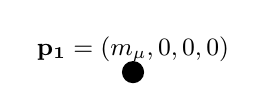
\begin{tikzpicture}[
        >=stealth,
        thick,
        every node/.style={font=\small}
    ]

        \coordinate (O) at (0,0);
        \fill (O) circle (4pt)
            node [above] {$\mathbf{p_1} = (m_\mu, 0, 0, 0)$}; 

    \end{tikzpicture}
    \end{center}

    \columnbreak

    \begin{center}
    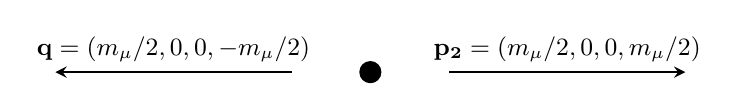
\begin{tikzpicture}[
        >=stealth,
        thick,
        every node/.style={font=\small}
    ]

        \coordinate (O) at (0,0);

        \draw[->] (-1,0) -- (-4, 0)
            node[midway, above] {$\mathbf{q} = (m_\mu/2, 0, 0, -m_\mu/2)$};

        \draw[->] (1,0) -- (4, 0)
            node[midway, above] {$\mathbf{p_2} = (m_\mu/2, 0, 0, m_\mu/2)$};

        % Vertice
        \fill (O) circle (4pt);

    \end{tikzpicture}
    \end{center}
    
\end{multicols}
\end{figure}

Avendo il modulo quadro, possiamo assemblare la larghezza di decadimento differenziale. Questa è data da 

\begin{align}
    d\Gamma = \frac{1}{2m_\mu}|\mathcal{\bar{M}}|^2dPS^{(2)}
\end{align}

L'elemento differenziale di spazio delle fasi \(dPS^{(2)}\) è lo stesso calcolato per lo scattering Bhabha, perché anche in questo caso abbiamo due particelle massless nello stato finale. 

\begin{align}
    dPS^{(2)} = \frac{d\Omega}{32\pi^2}
\end{align}

Segue quindi 

\begin{align}
    \frac{d\Gamma}{d\Omega} = \frac{2(f_1^2+f_2^2)m_\mu^4}{(2m_\mu)(32\pi^2)} \implies \Gamma = \int \frac{d\Gamma}{d\Omega}d\Omega = \frac{m^3_\mu (f_1^2+f_2^2)}{8\pi}
\end{align}

\subsection{Limiti sui fattori di forma}

Durante l'anno abbiamo calcolato la larghezza di decadimento \(\beta\) del muone, che ricordiamo: 

\begin{align}
    \Gamma(\mu^- \to e^- \nu_\mu \bar{\nu}_e) = \frac{G_F^2 m^5_\mu}{192\pi^2}
\end{align}

Da cui otteniamo una formula per il branching ratio: 

\begin{align}
    \text{BR}(\mu^-\to e^-\gamma) = \frac{\Gamma(\mu^-\to e^-\gamma)}{\Gamma(\mu^- \to e^- \nu_\mu \bar{\nu}_e)} = \left(\frac{(f_1^2+f_2^2)m_\mu^3}{8\pi} \right)\left(\frac{192\pi^2}{G_F^2 m_\mu ^5} \right) = \frac{24\pi (f_1^2+f_2^2)}{G_F^2 m_\mu^2} < 2.2 \cdot 10^{-13}
\end{align}

Possiamo definire \(F = \sqrt{f_1^2+f_2^2}\), e applicare dei limiti a questo fattore di forma, conoscendo \(G_F = 1.112 \cdot 10^{-5} \, \text{GeV}^{-2}\) e \(m_\mu = 106 \, \text{MeV} = 0.106\) GeV. Si ottiene così 

\begin{align}
    F = \frac{G_F m_\mu}{\pi}\sqrt{\frac{\text{BR}}{24}} < 3.59 \cdot 10^{-14} \, \text{GeV} 
\end{align}

\newpage

\section{Rinormalizzazione teoria di Yukawa}

Considera la seguente lagrangiana: 

\begin{align}
    \mathcal{L} = \bar{\psi}_0 (i\slashed{\partial} - m_{f0})\psi_0 + \frac{1}{2}(\partial\phi_0)^2 - \frac{1}{2}M_0^2\phi_0^2 - \lambda_0\bar{\psi_0}\psi_0 \phi_0
\end{align}

Come evidenziato dai pedici 0, la lagrangiana è scritta in termini di parametri "bare", non fisici. Risulta allora convieniente scriverla in termini di parametri fisici + dei controtermini, nel modo seguente: 

\begin{align}
    \mathcal{L} = &\bar{\psi}(i\slashed{\partial}-m_f)\psi + \frac{1}{2}(\partial\phi)^2 - \frac{M^2}{2}\phi^2 - \lambda \bar{\psi}\psi \phi \notag \\
    &+i\delta Z_\psi\bar{\psi}\slashed{\partial}\psi -i\delta m_f \bar{\psi}\psi + \frac{1}{2}\delta Z_\phi(\partial\phi)^2 - \frac{\delta M^2\phi^2}{2} - \delta \lambda \bar{\psi}\psi \phi 
\end{align}

Le regole di Feynman che risultano da questa lagrangiana sono le seguenti: 

\begin{multicols}{2}
    \begin{center}
        \begin{tikzpicture}
            \begin{feynman}
                \vertex (a); 
                \vertex [right = of a] (b); 
                \diagram{
                    (a) -- [fermion, momentum = \(p\)] (b); 
                }; 
            \end{feynman}
        \end{tikzpicture}
    \end{center}
    \columnbreak
    \begin{align}
        D_\psi(p) = \frac{i}{\slashed{p} - m_f + i\eps} 
    \end{align}
\end{multicols}

\begin{multicols}{2}
    \begin{center}
        \begin{tikzpicture}
            \begin{feynman}
                \vertex (a); 
                \vertex [right = of a] (b); 
                \diagram{
                    (a) -- [scalar, momentum = \(p\)] (b); 
                }; 
            \end{feynman}
        \end{tikzpicture}
    \end{center}
    \columnbreak
    \begin{align}
        D_\phi(p) = \frac{i}{p^2 - M^2 + i\eps} 
    \end{align}
\end{multicols}

\begin{multicols}{2}
    \begin{center}
        \begin{tikzpicture}
            \begin{feynman}
                \vertex (a); 
                \vertex [right = of a] (b); 
                \vertex [above left = of a] (c); 
                \vertex [below left = of a] (d); 
                \diagram{
                    (a) -- [scalar] (b); 
                    (c) -- [fermion] (a); 
                    (a) -- [fermion] (d); 
                }; 
            \end{feynman}
        \end{tikzpicture}
    \end{center}
    \columnbreak
    \begin{align}
        -i\lambda
    \end{align}
\end{multicols}

Usando queste, si calcolano i controtermini ordine per ordine in teoria delle perturbazioni, in modo tale che si verifichino le cosiddette \emph{condizioni di rinormalizzazione}. Nel nostro caso, vogliamo che valga: 

\begin{enumerate}
    \item La funzione a due punti della teoria deve sempre essere della forma 
    \begin{align}
        \frac{i}{p^2 - M^2 + i\eps}, \quad \frac{i}{\slashed{p} - m_f +i\eps}
    \end{align}
    A tutti gli ordini in teoria delle perturbazioni. 
    \item Nel limite in cui le tre particelle esterne sono on-shell, voglio che il vertice sia della forma 
    \begin{align}
        \Gamma_{\bar{\psi}\psi\phi} = -i\lambda
    \end{align}
\end{enumerate}

Al primo ordine in teoria delle perturbazioni, vediamo che le condizioni sono soddisfatte se i controtermini sono nulli. Il primo ordine non banale è quindi quello ad un loop. Indaghiamo nel dettaglio. 

\subsection{Campo spinoriale}

Considero i diagrammi di Feynman che contribuiscono alla funzione a due punti dello spinore, al livello di un loop. Un punto fondamentale è la determinazione della self energia, che corrisponde al diagramma in figura \ref{fig:selfenergyfermion}. Dalla condizione di rinormalizzazione già citata, oltre al propagatore standard, questa deve cancellare il contributo dei controtermini. Comincio allora il calcolo:   

\begin{figure}
    \caption{Contributo ad 1 loop della funzione a due punti del campo spinoriale}
    \label{fig:selfenergyfermion}
    \begin{center}
        \begin{tikzpicture}
            \begin{feynman}
                \vertex (a); 
                \vertex [right = of a] (b); 
                \vertex [right = of b] (c); 
                \vertex [right = of c] (d); 
                \diagram{
                    (a) -- [fermion, momentum' = \(p\)] (b); 
                    (b) -- [fermion, half right, momentum' = \(p+q\)] (c); 
                    (c) -- [scalar, half right, momentum' = \(q\)] (b); 
                    (c) -- [fermion, momentum' = \(p\)] (d); 
                }; 
            \end{feynman}
        \end{tikzpicture}
    \end{center}
\end{figure}


\begin{align}
    -i\Sigma(p) &= (-i\lambda)^2 \int \frac{d^4k}{(2\pi)^4}\int \frac{d^4k}{(2\pi)^4}\frac{i(\slashed{k}+m_f)}{k^2 - m_f^2}\frac{i}{(k-p)^2 - M^2} \notag \\ 
    &= \lambda^2\int \frac{d^4k}{(2\pi)^4}\frac{\slashed{k} + m_f}{(k^2-m^2_f)[(k-p)^2-M^2]}
\end{align}

Usiamo i parametri di Feynman per combinare i denominatori: 

\begin{align}
    -i\Sigma(p) &= \int_0^1 dx \int \frac{d^4k}{(2\pi)^4}\frac{\slashed{k}+m_f}{[-2xk\cdot p + xp^2 -xM^2 +k^2 -m^2_f +xm^2f]^2} \notag \\ 
    &= \lambda^2 \int_0^1 dx \int \frac{d^4k}{(2\pi)^4}\frac{(\slashed{k} + m_f)}{[(k-xp)^2 - \Delta]^2}
\end{align}

Cambio la variabile di integrazione, \(k \to \ell = k-xp\), 

\begin{align}
    -i\Sigma(p) &= \lambda^2\int_0^1 dx \int \frac{d^4\ell}{(2\pi)^4} \frac{x\slashed{p} + m_f}{[\ell^2 - \Delta]^2} \notag \\ 
    &= -i\lambda^2 \int_0^1 dx (x\slashed{p} + m_f)\int \frac{d^4\ell_E}{(2\pi)^4}\frac{1}{[\ell_E^2 + \Delta]^2}
\end{align}

Nell'ultimo passaggio abbiamo eseguito la rotazione di Wick. Per continuare con il conto usiamo la seguente formula: 

\begin{align}
    \int \frac{d^d\ell_E}{(2\pi)^d}\frac{1}{(\ell_E^2 + \Delta)^n} = \frac{\Delta^{d/2-n}}{(4\pi)^{d/2}}\frac{\Gamma(n-d/2)}{\Gamma(d/2)}
\end{align}

La formula si prova in modo diretto, calcolando l'integrale usando un paio di sostituzioni. 

\begin{align}
    \int \frac{d\Omega_{d-1}}{(2\pi)^d}\int \frac{d\ell_E \ell_E^{d-1}}{[\ell_E^2 + \Delta]^n} = \frac{1}{2}\int \frac{d\Omega_{d-1}}{(2\pi)^d}\int \frac{d(\ell_E^2)(\ell_E^2)^{\frac{d-2}{2}}}{[\ell_E^2 + \Delta]^n} 
\end{align}

Ora cambia la variabile \(\ell_E^2 \to y = \frac{\Delta}{\ell_E^2 + \Delta}\), così che \(\ell_E^2 = \frac{\Delta}{y} - \Delta\), \(d(\ell_E^2) = -\frac{\Delta}{y^2}dy\), e si ottiene 

\begin{align}
    &\int \frac{d\Omega_{d-1}}{(2\pi)^d}\int \frac{\Delta}{y^2}dy\left(\frac{y}{\Delta} \right)^n\Delta^{\frac{d-2}{2}}\left(\frac{1-y}{y} \right)^{\frac{d-2}{2}} =  \notag \\ 
    &\frac{\Delta^{\frac{d}{2}-n}}{2}\frac{2\pi^{d/2}}{\Gamma(d/2)}\int dy y^{n-1-d/2}(1-y)^{d/2-1}
\end{align}

L'ultimo integrale in \(dy\) ricorda la definizione integrale della funzione \(\beta\) di Eulero: 

\begin{align}
    \beta(\alpha, \gamma) = \int_0^1 dx x^{\alpha-1}(1-x)^{\gamma-1} = \frac{\Gamma(\alpha)\Gamma(\gamma)}{\Gamma(\alpha+\gamma)}
\end{align}

Sostituendo, troviamo la formula citata. Usando gli stessi passaggi si può anche dimostrare un altra formula che ci tornerà utile, 

\begin{align}
    \int \frac{d^d\ell_E}{(2\pi)^d}\frac{\ell_E^2}{(\ell_E^2 + \Delta)^n} = \frac{d}{2}\frac{\Delta^{d/2+1-n}}{(4\pi)^{d/2}}\frac{\Gamma(n-d/2-1)}{\Gamma(n)}
\end{align}

Tornando a noi, il diagramma \(-i\Sigma(p)\) è (logaritmicamente) divergente per \(d=4\). Adottiamo allora il sistema di regolarizzazione di riduzione dimensionale, e prendiamo \(d = 4-2\eps\) nel limite \(\eps \to 0\). La self energia dello spinore diventa quindi 

\begin{align}
    -i\Sigma(p) = -i\frac{\lambda^2}{(4\pi)^2}\int_0^1 dx [x\slashed{p} + m_f]\left(\frac{4pi\mu^2}{\Delta} \right)^\eps \Gamma(\eps)
\end{align}

Dove abbiamo riscalato \(\lambda \to \lambda\mu^\eps\) per tenerla adimensionale. Nel limite \(\eps \to 0\), otteniamo 

\begin{align}
    \left(\frac{4\pi\mu^2}{\Delta} \right)^\eps \Gamma(\eps) \xrightarrow{\eps \to 0} \left(1+\eps\log\left(\frac{4\pi\mu^2}{\Delta} \right) \right)\left(\frac{1}{\eps} + \gamma_E \right) = \frac{1}{\eps} + \gamma_E + \log\left(\frac{4\pi\mu^2}{\Delta} \right) + o(\eps)
\end{align}

Ovvero 

\begin{align}
    -i\Sigma(p) = -i\frac{\lambda^2}{(4\pi^2)}\int_0^1(x\slashed{p} +m_f)\left(\frac{1}{\eps} + \gamma_E + \log\left(\frac{4\pi\mu^2}{\Delta} \right) \right)
\end{align}

Se ci interessa solo la parte divergente, calcoliamo immediatamente 

\begin{align}
    -i\Sigma(p) = -i\frac{\lambda^2}{16\pi^2\eps}\left(\frac{\slashed{p}}{2} + m_f \right)
\end{align}

La condizione di rinormalizzazione chiede che questo contributo sia cancellato dai controtermini, cioè deve valere

\begin{align}
    -i\Sigma(p) = -i(\delta Z_\psi^2\slashed{p} - \delta m_f)
\end{align}

Possiamo calcolare quindi le parti infinite dei contotermini, uguagliando al lato destro e sinistro le potenze di \(\slashed{p}\): si ottiene 

\begin{align}
    \begin{cases}
        \delta Z_\psi = \frac{\lambda^2}{32\pi^2\eps} \\ 
        \delta m_f = -\frac{\lambda^2 m_f}{16\pi^2\eps}
    \end{cases}
\end{align}

\subsection{Campo scalare}

La stessa logica si applica al campo scalare. Richiediamo che valga 

\begin{align}
    \label{eq:scalarpropagatorrenormalizationcondition}
    -i\Sigma(p^2) = -i(\delta Z_\phi p^2 - \delta M)
\end{align}

dove con \(-i\Sigma(p^2)\) indichiamo la self energia dello scalare, corrispondente al diagramma di Feynman in figura \ref{fig:scalarselfenergy}. Calcoliamo l'ampiezza: 

\begin{figure}
    \caption{Self energia del campo scalare}
    \label{fig:scalarselfenergy}
    \begin{center}
        \begin{tikzpicture}
            \begin{feynman}
                \vertex (a); 
                \vertex [right = of a] (b); 
                \vertex [right = of b] (c); 
                \vertex [right = of c] (d); 
                \diagram{
                    (a) -- [scalar, momentum' = p] (b); 
                    (b) -- [fermion, half right, momentum' = p+q] (c);
                    (c) -- [fermion, half right, momentum' = q] (b); 
                    (c) -- [scalar, momentum' = p] (d); 
                }; 
            \end{feynman}
        \end{tikzpicture}
    \end{center}
\end{figure}


\begin{align}
    -i\Sigma(p^2) &= (-i\lambda)^2(-1)\int \frac{d^4q}{(2\pi)^4}\text{Tr}\left[\frac{i(\slashed{q}-\slashed{p}+m_f)}{[(q-p)^2 - m_f^2]}\frac{i(\slashed{q}+m_f)}{q^2-m^2_f}\right] \notag \\ 
    &= -4\lambda^2 \int \frac{d^4q}{(2\pi)^4}\frac{m_f^2 + (q-p)\cdot p}{[(q-p)^2 - m^2_f][q^2 - m^2_f]}
\end{align}

Come al solito, uso i parametri du Feynman e cambio variabile di integrazione: 

\begin{align}
    -i\Sigma(p^2) &= -4\lambda^2 \int_0^1 dx \int  \frac{d^4q}{(2\pi)^4}\frac{m_f^2 + (q-p)\cdot q}{[xp^2 - 2xp\cdot q + q^2 - m^2_f]^2} \notag \\ 
    &= -4\lambda^2 \int_0^1 dx \int \frac{d^4q}{(2\pi)^4}\frac{m^2_f + (q-p)\cdot q}{[(q-xp)^2 - \Delta]^2}, \quad \Delta = m^2_f - (1-x)xp^2 \notag \\ 
    &= -4\lambda^2 \int_0^1 dx \int \frac{d^4\ell}{(2\pi)^4}\frac{\ell^2 + \Delta}{[\ell^2 - \Delta]^2}, \quad \ell = q-xp \notag \\ 
    &= -4\lambda^2 \int_0^1dx (I_1 + \Delta I_2)
\end{align}

Se definiamo 

\begin{align}
    &I_1 = \int \frac{d^4\ell}{(2\pi)^4}\frac{\ell^2}{[\ell^2 - \Delta]^2} = \frac{2i\Delta}{(4\pi)^2}\left(\frac{4\pi\mu^2}{\Delta} \right)^\eps\Gamma(-1+\eps) \notag \\ 
    &I_2 = \int \frac{d^4\ell}{(2\pi)^4}\frac{1}{[\ell^2 - \Delta]^2} = \frac{-i}{(4\pi)^2}\left(\frac{4\pi\mu^2}{\Delta} \right)^\eps \Gamma(\eps)
\end{align}

Dove abbiamo usato le formule precedentemente usate. Quindi, troviamo 

\begin{align}
    -i\Sigma(p^2) &= -4i\lambda^2 \int_0^1 dx \left[\frac{2\Delta}{(4\pi)^2}\left(\frac{4\pi\mu^2}{\Delta}\right)^\eps\Gamma(-1+\eps) - \frac{\Delta}{(4\pi)^2}\left( \frac{4\pi\mu^2}{\Delta}\right)^\eps \Gamma(\eps) \right] \notag \\ 
    &= -\frac{i\lambda^2}{4\pi^2}\int_0^1 dx \Delta \left(\frac{4\pi\mu^2}{\Delta} \right)^\eps(2\Gamma(-1+\eps) - \Gamma(\eps))
\end{align}

Se ci fermiamo allo sviluppo di Laurent in \(\eps\) fino all'ordine zero, troviamo 

\begin{align}
    -i\Sigma(p^2) &= -\frac{i\lambda^2}{4\pi^2}\int_0^1 dx \Delta \left(1+\eps\log\left(\frac{4\pi\mu^2}{\Delta}\right) \right)\left(-\frac{2}{\eps} + 2\gamma_E - 2 - \frac{1}{\eps} - \gamma_E \right) \notag \\ 
    &= -\frac{i\lambda^2}{4\pi^2}\int_0^1 dx \Delta \left[-\frac{3}{\eps} - 2+\gamma_E -2\log\left(\frac{4\pi\mu^2}{\Delta} \right)\right]
\end{align}

Se ci interessa solo la parte infinita dei controtermini, possiamo prendere 

\begin{align}
    -i\Sigma(p^2) &= i\frac{\lambda^2}{4\pi^2}\frac{3}{\eps}\int_0^1 dx \Delta + 0(1) \notag \\ 
    &= i\frac{3\lambda^2}{4\pi^2\eps}\left(m_f^2 - \frac{p^2}{6}\right) + o(1)
\end{align}

Applicando quindi la condizione di rinormalizzazione \ref{eq:scalarpropagatorrenormalizationcondition}, otteniamo 

\begin{align}
    \begin{cases}
        \delta Z_\phi = -\frac{\lambda^2}{8\pi^2\eps} \\
        \delta m = -\frac{3\lambda^2}{4\pi^2\eps}
    \end{cases}
\end{align}

\subsection{Costante di accoppiamento}

L'ultimo passaggio del calcolo dei controtermini al primo ordine perturbativo è il calcolo del controtermine di carica \(\delta \lambda\). La condizione di rinormalizzazione che scegliamo è la seguente: il vertice deve essere quello misurato \(-i\lambda\) nel limite in cui tutte le particelle esterne sono on-shell. Chiramente a livello d'albero la condizione è soddisfatta se \(\delta \lambda^{(0)} = 0\). Invece, a livello di 1 loop, le correzioni al vertice sono molteplici: ci sono i contributi di self energia, che vengono però perfettamente cancellati dai controtermini di massa e di funzione d'onda. I 3 contributi che rimangono sono dunque vertice ad albero, vertice del controtermine e vertice "triangolo", dato dal diagramma di Feynman in figura \ref{fig:trianglediagram}. Se indichiamo con \(iA\) l'ampiezza di quest'ultimo, si ottiene che la condizione di rinormalizzazione è data da 

\begin{align}
    -i\lambda -i\delta \lambda^{(1)} +iA(m_f^2, m_f^2, M^2) = -i\lambda \implies \delta \lambda^{(1)} = A(m_f^2, m_f^2, M^2)
\end{align}

Calcolo dunque l'ampiezza \(iA\) del diagramma a triangolo: \footnote{Abbiamo scelto i momenti in modo tale che semplicassero il più possibile le masse nel calcolare l'ampiezza on-shell}

\begin{figure}
    \caption{Diagramma a triangolo che contribuisce a \(\Gamma_{\bar{\psi}\psi \phi}\) al secondo ordine perturbativo}
    \label{fig:trianglediagram}
    \begin{center}
            \begin{tikzpicture}
                \begin{feynman}
                    \vertex (a); 
                    \vertex [above left = of a] (b); 
                    \vertex [below left = of a](c); 
                    \vertex [right = of a] (d); 
                    \vertex [left = of b] (e); 
                    \vertex [left = of c] (f); 
                    \diagram{
                        (b) -- [fermion] (a); 
                        (a) -- [fermion] (c); 
                        (a) -- [scalar] (d); 
                        (b) -- [scalar] (c); 
                        (e) -- [fermion] (b); 
                        (c) -- [fermion] (f); 
                    }; 
                \end{feynman}
            \end{tikzpicture}
        \end{center}
\end{figure}

\begin{align}
    iA(m^2, m^2, M^2) &= (-i\lambda)^3 \int \frac{d^4k}{(2\pi)^4}\left[\frac{i(\slashed{k} + \slashed{p_1} +m)}{(k+p_1)^2-m^2} \right]\left[\frac{i(\slashed{k}-\slashed{p_2}+m)}{(k-p_2)^2-m^2} \right]\left[\frac{i}{k^2-M^2} \right] \notag \\ 
    &= -\lambda^3 \int \frac{d^4k}{(2\pi)^4}\frac{(\slashed{k} + \slashed{p_1} + m)(\slashed{k} -\slashed{p_2} + m)}{[k^2 + 2k\cdot p_1][k^2 - 2k\cdot p_2][k^2-M^2]}
\end{align}

Notiamo che ho tre denominatori, quindi è necessario usare due parametri di Feynman. In particolare usiamo la formula

\begin{align}
    \frac{1}{ABC} = 2\int_0^1dx\int_0^{1-x}dy \frac{1}{[xA + yB + (1-x-y)C]^3}
\end{align}

Scegli \(C = k^2-M^2, \, A = k^2 + 2k\cdot p_1, \, B = k^2 - 2k\cdot p_2\). Il denominatore diventa: 

\begin{align}
    \text{Den} &= 2xk\cdot p_1 -2y k\cdot p_2 + k^2 - M^2 -xM^2 -yM^2 \notag \\
    &= (k + xp_1 - yp_2)^2 - \underbrace{[(xp_1 - yp_2)^2 +(1-x-y)M^2]}_{=\Delta} 
\end{align}

L'ampiezza è quindi data da 

\begin{align}
    iA = -2\lambda^3 \int_0^1 dx\int_0^{1-x} dy\int \frac{d^4k}{(2\pi)^4}\frac{(\slashed{k}+ \slashed{p_1} +m)(\slashed{k}- \slashed{p_2} +m)}{[(k+xp_1 - yp_2)^2 - \Delta]^3}
\end{align}

Facciamo quindi la sostituzione \(k \to \ell = k+xp_1 - yp_2\), e otteniamo così 

\begin{align}
    iA = -2\lambda^3 \int_0^1dx \int_0^{1-x} dy \int \frac{d^4\ell}{(2\pi)^4}\frac{(\slashed{\ell} + (x+1)\slashed{p_1} - y\slashed{p_2} + m)(\slashed{\ell} + x\slashed{p_1} - (y+1)\slashed{p_2} + m)}{[\ell^2 - \Delta]^3}
\end{align}

Teniamo solo i contributi di ordine 0 e 2 in \(\ell\), che non si cancellano per parità: 

\begin{align}
    iA = -2\lambda^3\int_0^1 dx \int_0^{1-x} dy \int \frac{d^4\ell}{(2\pi)^4} &\frac{\ell^2 + x(x+1)m^2 -(x+1)(y+1)\slashed{p_1}\slashed{p_2} + m(x+1)\slashed{p_1}}{[\ell^2 - \Delta]^3} \notag \\ 
    &+ \frac{-xy\slashed{p_2}\slashed{p_1} +y(y+1)m^2 -ym\slashed{p_2} + xm\slashed{p_1} - (y+1)m\slashed{p_2} +m^2}{[\ell^2 -\Delta]^3}
\end{align}

Che prende la forma 

\begin{align}
    iA = -2\lambda^3 \int_0^1 dx \int_0^{1-x} dy (&I_1 + (m^2(1 + x(x+1) + y(y+1)) + \notag \\ 
    &m((2x+1)\slashed{p_1} - (2y+1)\slashed{p_2}) -((x+1)(y+1)\slashed{p_1}\slashed{p_2} + xy\slashed{p_2}\slashed{p_1}))I_2)
\end{align}

Se abbiamo definito

\begin{align}
    I_1 &= \int \frac{d^4\ell}{(2\pi)^4}\frac{\ell^2}{[\ell^2 -\Delta]^3} = -i\int \frac{d^4\ell_E}{(2\pi)^4}\frac{\ell_E^2}{[\ell_E^2+\Delta]^3} \notag \\ &= -\frac{i\Gamma(\eps)}{(4\pi)^2}\left(\frac{4\pi\mu^2}{\Delta} \right)^\eps \xrightarrow{\eps \to 0} -\frac{i}{16\pi^2}\left[\frac{1}{\eps} + \gamma_E + \log\left(\frac{4\pi\mu^2}{\Delta}\right) \right]
\end{align}

e similmente 

\begin{align}
    I_2 &= \int \frac{d^4\ell}{(2\pi)^4}\frac{1}{[\ell^2-\Delta]^3} = i\int \frac{d^4\ell_E}{(2\pi)^4}\frac{1}{[\ell_E^2 + \Delta]^3} \notag \\ 
    &= \frac{i}{2\Delta(4\pi)^2}\left(\frac{4\pi\mu^2}{\Delta} \right)^\eps \Gamma(1+\eps) \xrightarrow{\eps \to 0}  \frac{i}{32\pi^2\Delta}
\end{align}

Come ci si aspetta anche dal grado superficiale di divergenza, vediamo che \(I_1\) diverge logaritmicamente mentre \(I_2\) è UV finito. 

Fortunatamente dobbiamo calcolare esplicitamente solamente la parte divergente dell'integrale, mentre possiamo lasciare indicata simbolicamente le parti finite. La parte divergente è quindi data da 

\begin{align}
    iA = 2\int_0^1 dx \int_0^{1-x}dy \frac{i\lambda^3 }{16\pi^2 \eps} + o(1) =  \frac{i\lambda^3 }{16\pi^2 \eps} + o(1) \quad \eps \to 0 
\end{align}

Concludiamo quindi che 

\begin{align}
    \delta \lambda^{(1)} = A = \frac{\lambda^3}{16\pi^2 \eps}
\end{align}

\subsection{Controtermini in diversi schemi di rinormalizzazione}

Nel caso in cui volessi usare diverse schemi di rinormalizzazione, i controtermini sono leggermente diversi. Ad esempio mettiamo io voglia calcolare i controtermini usando lo schema on-shell: è facile vedere che con le nostre convenzioni, deve valere 

\begin{align}
    &\delta M^2 = -\Sigma_\phi(M^2) \notag \\ 
    &Z_\phi = \frac{1}{1-\Sigma_\phi'(p^2 = M^2)} \simeq \Sigma'(p^2 = M^2)\notag \\
    &\delta m_f = \Sigma_\psi (m_f) \notag \\ 
    &Z_\psi = \frac{1}{1-\Sigma'(p = m_f)} \simeq \Sigma'(p = m_f)
\end{align}

Date le espressioni già calcolate, è facile vedere che 

\begin{align}
    &\Sigma_\phi (M^2) = \frac{3\lambda^2}{4\pi^2\eps}[m_{f,0}^2 - \frac{M^2}{6}] \notag \\ 
    &\Sigma'_\phi(p^2 = M^2) = \frac{\lambda^2}{8\pi^2\eps} \notag \\ 
    &\Sigma_\psi(\slashed{p} = m_f) = \frac{3m_f\lambda^2}{32\pi^2\eps}
\end{align}

Per la self energia del fermione, ricorda che vale 

\begin{align}
    \Sigma_\psi (\slashed{p}) = A(p^2, m)\mathbb{I} + B(p^2, m)\slashed{p} \implies \frac{\partial \Sigma_\psi}{\partial \slashed{p}} = 2\slashed{p}\frac{\partial A}{\partial p^2} + B + 2p^2\frac{\partial B}{\partial p^2}
\end{align}


Nel nostro caso, \(B = A/2 = \frac{\lambda^2}{32\pi^2\eps}\). Si trova quindi 

\begin{align}
    \Sigma'_\psi = \frac{\lambda^2}{32\pi^2\eps}
\end{align}

\newpage 

\section{Nuova fisica nel decadimento del muone}

Consideriamo adesso un'estensione del Modello Standard, in cui è possibile il decadimento del muone 

\begin{align}
    \mu^- \to e^- \, \gamma
\end{align}

Consiste nell'aggiunta di un campo scalare carico \(\phi^+\), e di un fermione \(\Psi\), con massa rispettivamente \(M_\phi, M_\Psi\). La lagrangiana di interazione con il campo del fotone, elettrone e muone è data da 

\begin{align}
    \mathcal{L}_{\text{int}} = (D_\nu \phi^+)(D^\nu \phi^+)^* + y_e (\bar{\Psi}\psi_e \phi^+ + \, \text{h.c.}) + y_\mu (\bar{\Psi}\psi_\mu \phi^+ + \, \text{h.c.})
\end{align}

se \(D_\nu = \partial_\nu + ieA_\nu\), cioè la derivata covariante rispetto alle trasformazioni di gauge \(U(1)\) dell'elettromagnetismo. 

\subsection{Regole di Feynman della teoria}

Questa lagrangiana di interazione permette l'aggiunta di 4 vertici al modello standard. I diagrammi di Feynman corrispondenti sono in figura \ref{fig:newvertexes}. 

\begin{figure}
    \caption{Nuovi vertici aggiunti dall'estensione}
    \label{fig:newvertexes}
    \begin{multicols}{4}
        \begin{center}
            \begin{tikzpicture}
                \begin{feynman}
                    \vertex (a); 
                    \vertex [above left = of a] (b) {\(\bar{\Psi}\)}; 
                    \vertex [below left = of a] (c) {\(e^-\)}; 
                    \vertex [right = of a] (d) {\(\phi^+\)}; 
                    \diagram{
                        (c) -- [fermion] (a); 
                        (a) -- [fermion] (b); 
                        (a) -- [scalar] (d); 
                    }; 
                \end{feynman}
            \end{tikzpicture}
        \end{center}
    \columnbreak
        \begin{center}
            \begin{tikzpicture}
                \begin{feynman}
                    \vertex (a); 
                    \vertex [above left = of a] (b) {\(\bar{\Psi}\)}; 
                    \vertex [below left = of a] (c) {\(\mu^-\)}; 
                    \vertex [right = of a] (d) {\(\phi^+\)}; 
                    \diagram{
                        (c) -- [fermion] (a); 
                        (a) -- [fermion] (b); 
                        (a) -- [scalar] (d); 
                    }; 
                \end{feynman}
            \end{tikzpicture}
        \end{center}
    \columnbreak
        \begin{center}
            \begin{tikzpicture}
                \begin{feynman}
                    \vertex (a); 
                    \vertex [above left = of a] (b) {\(\phi^{+*}\)}; 
                    \vertex [below left = of a] (c) {\(\phi^+\)}; 
                    \vertex [right = of a] (d) {\(A_\mu\)}; 
                    \diagram{
                        (c) -- [scalar] (a); 
                        (a) -- [scalar] (b); 
                        (a) -- [boson] (d); 
                    }; 
                \end{feynman}
            \end{tikzpicture}
        \end{center}
    \columnbreak
        \begin{center}
            \begin{tikzpicture}
                \begin{feynman}
                    \vertex (a); 
                    \vertex [above left = of a] (b) {\(\phi^{+*}\)}; 
                    \vertex [below left = of a] (c) {\(\phi^+\)}; 
                    \vertex [above right = of a] (d) {\(A_\mu\)}; 
                    \vertex [below right = of a] (e) {\(A_\nu\)}; 
                    \diagram{
                        (c) -- [scalar] (a); 
                        (a) -- [scalar] (b); 
                        (a) -- [boson] (d); 
                        (a) -- [boson] (e); 
                    }; 
                \end{feynman}
            \end{tikzpicture}
        \end{center}
    \end{multicols}
\end{figure}

Sempre dalla lagrangiana leggiamo le regole di Feynman: in particolare, troviamo: 

\begin{align}
    \Gamma_{\bar{\psi}\psi_e \phi^+} = -iy_e, \quad \Gamma_{\bar{\psi}\psi_\mu \phi^+} = -iy_\mu
\end{align}

Per ricavare quelle per l'interazione fra il campo scalare e il campo elettromagnetico, sviluppo la derivata covariante: 

\begin{align}
    (D_\nu \phi^+)(D^\nu \phi^+)^* &= (\partial_\nu \phi^+ +ieA_\nu \phi^+)(\partial^\nu \phi^{+*} -ieA^\nu \phi^{+*}) \notag \\
    &= (\partial_\nu \phi^+)(\partial^\nu \phi^+)^* +ieA_\nu (\phi^+(\partial_\nu \phi^+)^* - \phi^{+*}(\partial_\nu\phi^+)) + e^2 A_\nu A^\nu |\phi^+|^2
\end{align}

Ricordando quindi che siamo nello spazio dei momenti e possiamo sostituire \(\partial_\mu \to ip_\mu\), e che nel vertice a 4 dobbiamo moltiplicare per un fattore 2, data la simmetria dei bosoni vettori esterni, si trova 

\begin{align}
    \Gamma_{\phi^+ \phi^{+*} A_\mu} = ie(p_2-p_1)^\mu, \quad \Gamma_{\phi^+ \phi^{+*} A_\mu A_\nu} = 2ie^2 g^{\mu\nu}
\end{align}

\subsection{Contributo al fattore di forma}

Consideriamo ancora il decadimento \(\mu^- \to e^- \gamma\). Esistono 3 diagrammi ad un loop nella nostra teoria che rendono possibile il processo, illustrati in figura \ref{fig:muongammadecayfeynman}. Poichè la teoria conserva la parità, è chiaro, dalle considerazioni dell'esercizio sul decadimento del muone, che la struttura totale della ampiezza dovrà essere della forma \(\mathcal{M}^\mu = \bar{u}_e(p_2)[if_1 \sigma^{\mu\nu}q_\nu] u_\mu (p_1)\). Tra questi, i due diagrammi di self energia sono \(\propto \gamma^\mu\), e divergenti. Non contribuiscono dunque ad \(f_1\), ma solo il diagramma "a triangolo" lo fa. Vediamo dunque di esprimere il fattore di forma \(f_1\) proprio in termini di integrali di loop.    

\begin{figure}
    \caption{Diagrammi di Feynman per il decadimento \(\mu^- \to e^- \gamma\)}
    \label{fig:muongammadecayfeynman}
    \begin{center}
        \begin{tikzpicture}
            \begin{feynman}
                \vertex (a) {\(\mu^-\)}; 
                \vertex [right = of a] (b); 
                \vertex [above right = of b] (c); 
                \vertex [right = of c] (d) {\(e^-\)};  
                \vertex [below right = of c] (e); 
                \vertex [right = of e] (f) {\(A_\mu\)}; 
                \diagram{
                    (a) -- [fermion] (b); 
                    (b) -- [fermion, edge label = \(\Psi\)] (c); 
                    (c) -- [fermion] (d); 
                    (c) -- [scalar, edge label = \(\phi^+\)] (e); 
                    (b) -- [scalar, edge label = \(\phi^{+*}\), half right] (e); 
                    (e) -- [boson] (f); 
                }; 
            \end{feynman}
        \end{tikzpicture}
        \begin{tikzpicture}
            \begin{feynman}
                \vertex (a) {\(\mu^-\)}; 
                \vertex [right = of a] (b); 
                \vertex [right = of b] (c); 
                \vertex [right = of c] (d); 
                \vertex [above right = of d] (e) {\(e^-\)}; 
                \vertex [below right = of d] (f) {\(A_\mu\)}; 
                \diagram{
                    (a) -- [fermion] (b); 
                    (b) -- [fermion, half left, edge label = \(\Psi\)] (c);
                    (b) -- [scalar, half right, edge label' = \((\phi^+)^*\)] (c); 
                    (c) -- [fermion] (d); 
                    (d) -- [fermion] (e); 
                    (d)  -- [boson] (f); 
                }; 
            \end{feynman}
        \end{tikzpicture}
        \begin{tikzpicture}
            \begin{feynman}
                \vertex (a) {\(\mu^-\)}; 
                \vertex [right = of a] (b); 
                \vertex [above right = of b] (c); 
                \vertex [below right = of b] (d) {\(A_\mu\)}; 
                \vertex [right = of c] (e); 
                \vertex [right = of e] (f) {\(e^-\)}; 
                \diagram{
                    (a) -- [fermion] (b); 
                    (b) -- [fermion, edge label = \(\mu^-\)] (c);
                    (b) -- [boson] (d); 
                    (c) -- [fermion, half left, edge label = \(\Psi\)] (e); 
                    (c) -- [scalar, half right, edge label' = \((\phi^+)^*\)] (e); 
                    (e) -- [fermion] (f); 
                }; 
            \end{feynman}
        \end{tikzpicture}
    \end{center}
\end{figure}

Chiamiamo la ampiezza totale \(\mathcal{M}^\mu = \mathcal{M}^\mu_1 +\mathcal{M}^\mu_2 + \mathcal{M}^\mu_3\). Usando le regole di Feynman troviamo (supponendo che valga \(M = M_\Psi = M_\phi\))

\begin{align}
    &\mathcal{M}^\mu_1 = \bar{u}_e(p_2)(y_ey_\mu e) \left(\int \frac{d^4k}{(2\pi)^4}\frac{(-2k + p_1 + p_2)^\mu (\slashed{k}+M)}{[(k-p_1)^2 - M^2][(k-p_2)^2 - M^2][k^2 - M^2]}\right) u_\mu (p_1) \notag \\
    &\mathcal{M}^\mu_2 = \bar{u}_e(p_2)(y_e y_\mu e)\gamma^\mu \frac{\slashed{p}_1}{m^2_\mu}\left(\int \frac{d^4k}{(2\pi)^4}\frac{\slashed{k}+M}{[k^2-M^2][(k-p_1)^2 - M^2]} \right)u_\mu (p_1) \notag \\
    &\mathcal{M}^\mu_3 = -\bar{u}_e(p_2)(ey_e y_\mu)\left(\int \frac{d^4k}{(2\pi)^4}\frac{\slashed{k} + M}{[k^2 - M^2][(k-p_2)^2 - M^2]} \right)\frac{\slashed{p}_2 + m_\mu}{m_\mu^2}\gamma^\mu u_\mu (p_1)
\end{align}

Cominciamo il calcolo manipolando la ampiezza del diagramma a triangolo, cioè \(\mathcal{M}_1^\mu\). In particolare, vogliamo scriverlo nella base che abbiamo indicato di matrici di Dirac (cioè \(\gamma^\mu, q^\mu, \sigma^{\mu\nu}q_\nu\)). Dopodiché, le parti \(\propto q^\mu\) si cancellano perché si contraggono con il vettore di polarizzazione del fotone esterno, \(\eps^*(q)\). La parte invece \(\propto \gamma^\mu\) deve cancellare il contributo delle self energie, in modo che rimanga solamente la struttura \(\propto \sigma^{\mu\nu}q_\nu\), che è proprio il fattore di forma \(f_1\) da noi cercato. 

Per prima cosa, mostrerò come scrivere \(\mathcal{M}_1^\mu\) in termini di \(\gamma^\mu, \sigma^{\mu\nu}q_\nu\). Poi per completezza mostrerò che le parti \emph{UV divergenti} dell'ampiezza si cancellano, così che la ampiezza sia finita. Questo è un test non banale sulla scrittura corretta della ampiezza. Per le parti finite invece ci fideremo dell'identità di Ward. Successivamente, potremo isolare il fattore di forma \(f_1\), in termini di integrali sui parametri di Feynman su funzioni razionali. 

Chiamiamo \(I\) l'integrale di loop in \(\mathcal{M}_1\). Introduciamo i parametri di Feynman: 

\begin{align}
    I &= 2\int_0^1 dx \int_0^{1-x}dy \int \frac{d^4k}{(2\pi)^4}\frac{(-2k + p_1 + p_2)^\mu (\slashed{k}+M)}{[-2xk\cdot p_1 +xm_\mu^2 -2k\cdot p_2 +k^2 -M^2]^3} \notag \\
    &= 2\int_0^1 dx \int_0^{1-x}dy \int \frac{d^4k}{(2\pi)^4}\frac{(-2k + p_1 + p_2)^\mu (\slashed{k}+M)}{(k-xp_1 -yp_2)^2 -M^2 -xym_\mu^2 -x(1-x)m^2_\mu} \notag \\ 
    &= 2 \int_0^1 dx \int_0^{1-x}dy \int \frac{d^4\ell}{(2\pi)^4}\frac{(-2k + (1-2x)p_1 + (1-2y)p_2)^\mu (\slashed{\ell} + xm_\mu + M)}{[\ell^2 - \Delta]^3}
\end{align}

Nell'ultimo passaggio abbiamo cambiato variabile di integrazione \(k \to \ell = k - xp_1 - yp_2\), definito \(\Delta = M^2 + xym_\mu^2 + x(1-x)m_\mu^2\), ed usato l'eq. di Dirac, \(\bar{u}_\mu(p_1)\slashed{p_1} = \bar{u}_\mu (p_1)m_\mu\), ed \(\slashed{P_1}u_e(p_1) = 0\). Per parità soppravvivono nell'integrale solo le componenti \(\propto \ell^2, \, \ell^0\): 

\begin{align}
    I = 2\int_0^1 dx \int_0^{1-x}dy \int \frac{d^4\ell}{(2\pi)^4}\frac{-2\ell^\mu \slashed{\ell} + ((1-2x)p_1 + (1-2y)p_2)^\mu(xm_\mu +M)}{[\ell^2 - \Delta]^3}
\end{align}

Immediatamente vediamo che il diagramma ha una parte logaritmicamente divergente, ed una parte convergente. La parte divergente è \(\propto \gamma^\mu\), e serve per cancellare le divergenze dei diagrammi con le self-energie. Vediamolo esplicitamente: 

\begin{align}
    \label{eq:infinitetriangle}
    I' &= -4 \gamma_\nu \int_0^1 dx \int_0^{1-x}dy \int \frac{d^4\ell}{(2\pi)^4}\frac{\ell^\mu \ell^\nu}{[\ell^2 -\Delta]^3} = -\frac{4}{d} \gamma^\mu \int_0^1 dx \int_0^{1-x}dy \int \frac{d^4\ell}{(2\pi)^4}\frac{\ell^2}{[\ell^2 -\Delta]^3} \notag \\ 
    &= \frac{4i}{d}\int_0^1 dx \int_0^{1-x}dy \int \frac{d^4\ell}{(2\pi)^4}\frac{\ell_E^2}{[\ell_E^2 + \Delta]^3} = \frac{2i}{d}\gamma^\mu \frac{d}{2}\frac{\Gamma(\eps)}{2(4\pi)^2} = \frac{i\gamma^\mu}{32\pi^2\eps} + o(1)
\end{align}

Per calcolare le ampiezze degli altri due diagrammi, comincio con il sottodiagramma della self energia: 

\begin{align}
    -i\Sigma(p) &= (y_e y_\mu) \int \frac{d^4k}{(2\pi)^4}\frac{\slashed{k}+M}{(k^2 -M^2)((k-p)^2 - M^2)} \notag \\ 
    &= (y_e y_\mu) \int_0^1 dx \int \frac{d^4k}{(2\pi)^4}\frac{\slashed{k}+M}{[xp^2 -2xp\cdot k + k^2 - M^2]^2} \notag \\ 
    &= (y_e y_\mu) \int_0^1 dx \int \frac{d^4\ell}{(2\pi)^4}\frac{x\slashed{p} + M}{[\ell^2 - \Delta]^2}
\end{align}

Dove abbiamo cambiato variabile di integrazione \(k \to \ell = k-xp\), chiamato \(\Delta = M^2 -x(1-x)p^2\). Proseguendo con il calcolo, otteniamo 

\begin{align}
    -i\Sigma(p) &= (y_e y_\mu)\int_0^1 dx (x\slashed{p} + M)\int \frac{d^4\ell}{(2\pi)^4}\frac{1}{[\ell^2 - \Delta]^2} = -i(y_e y_\mu) \int_0^1 dx (x\slashed{p} + M)\int \frac{d^4\ell_E}{(2\pi)^4}\frac{1}{[\ell_E^2 + \Delta]^2} \notag \\ 
    &= \frac{-iy_e y_\mu}{(4\pi)^2\eps}\left(\frac{\slashed{p}}{2} +M \right) +o(1)
\end{align}

Possiamo allora facilmente calcolare la parte infinita dell'ampiezza dei diagrammi di self energia: 

\begin{align}
    \mathcal{M}_2^\mu = \bar{u}_e (-ie\gamma^\mu)\frac{i\slashed{p_1}}{m^2_\mu}(-i\Sigma(p_1))u_\mu (p_1)
\end{align}

Usando l'eq. di Dirac e semplificando, si ottiene facilmente 

\begin{align}
    \mathcal{M}_2^\mu = -i\frac{ey_e y_\mu}{(4\pi)^2\eps}\left(\frac{1}{2} + \frac{M}{m_\mu} \right)\bar{u}_e(p_2)
\end{align}

Svolgiamo gli stessi passaggi per il terzo diagramma: 

\begin{align}
    \mathcal{M}_3^\mu &= \bar{u}_e(p_2)(-i\Sigma(p_2))\frac{i(\slashed{p_2}+m_\mu)}{-m_\mu^2}(-ie\gamma^\mu)u_\mu(p_1) \notag \\
    &= i\frac{e y_e y_\mu}{(4\pi)^2\eps}\left(\frac{\slashed{p}_2}{2}+M \right)\left(\frac{\slashed{p}_2 + m_\mu}{m_\mu^2} \right)\gamma^\mu u_\mu (p_1) \notag \\ 
    &= i\frac{e y_e y_\mu}{(4\pi)^2\eps}\left(\frac{M}{m_\mu} \right)\bar{u}_e(p_2)\gamma^\mu u_\mu(p_1)
\end{align}

Troviamo quindi 

\begin{align}
    \mathcal{M}_2^\mu + \mathcal{M}_3^\mu = -i\frac{e y_e y_\mu}{32\pi^2\eps}\bar{u}_e(p_2)\gamma^\mu u_\mu (p_1) + o(1)
\end{align}

che è esattamente l'opposto del termine infinito calcolato da \(\mathcal{M}_1^\mu\) (eq. \ref{eq:infinitetriangle}). 

Avendo verificato che l'identità di Ward funziona per i termini \(\propto \eps^{-1}\), ci fidiamo che cancelli anche i termini finiti, proprizionali a \(\gamma^\mu\). Torniamo quindi a considerare la parte convergente rimasta dell'integrale: 

\begin{align}
    I'' = 2\int_0^1 dx \int_0^{1-x}dy \int \frac{d^4\ell}{(2\pi)^4}\frac{(xm_\mu +M)((1-2x)p_1^\mu + (1-2y)p_2^\mu)}{[\ell^2 -\Delta]^3}
\end{align}

Si calcola subito l'integrale in \(\ell\): 

\begin{align}
    I'' = \frac{i}{(4\pi)^2}\int_0^1 dx \int_0^{1-x}dy \frac{(M+xm_\mu)((1-2x)p_1^\mu + (1-2y)p_2^\mu)}{\Delta}
\end{align}

Scrivo \(p_1, p_2\) in termini di \(p = p_1+p_2\), \(q = p_1-p_2\) (cioè usando \(p_1 = (p+q)/2\) ed \(p_2 = (p-q)/2\)). Questo è conveniente perchè i pezzi \(\propto q^\mu\) si contraggono e si cancellano con il vettore di polarizzazione del fotone esterno, \(\eps_\mu(q)\). Si ottiene così 

\begin{align}
    I'' = i\frac{p_1^\mu + p_2^\mu}{16\pi^2}\int_0^1 dx \int_0^{1-x}dy \frac{(M+xm_\mu)(1-x-y)}{\Delta}
\end{align}

Posso ora usare l'identità di Gordon, e scartare il termine \(\propto \gamma^\mu\). Si ottiene allora una espressione per la ampiezza totale: 

\begin{align}
    i\mathcal{M}^\mu = i \bar{u}_e(p_2)\left[\frac{-i(ey_ey_\mu)\sigma^{\mu\nu}q_\nu}{16\pi^2}\int_0^1 dx \int_0^{1-x}dy \frac{(M+xm_\mu)(1-x-y)}{\Delta}\right]u_\mu (p_1)
\end{align}

Confrontando l'espressione con \(\mathcal{M}^\mu = i\bar{u}_e(p_2)f_1\sigma^{\mu\nu}q_\nu u_\mu(p_1)\), si legge immediatamente 

\begin{align}
    f_1 = -\frac{(ey_e y_\mu)}{16\pi^2}\int_0^1 dx \int_0^{1-x}dy \frac{(M+xm_\mu)(1-x-y)}{\Delta}
\end{align}

\subsection{Calcolo esplicito degli integrali di loop}

Per determinare \(f_1\), devo calcolare il doppio integrale in \(x, y\). L'integranda è una funzione razionale, del primo grado in \(y\) e del secondo grado in \(x\). L'integrazione è certamente possibile quindi ma anche poco gradevole. Esplicitando \(\Delta\), l'integrale da risolvere è dato da 

\begin{align}
    \int_0^1 dx \int_0^{1-x}dy \frac{(M+xm_\mu)(1-x-y)}{M^2 +xym^2_\mu - x(1-x)m^2_\mu}
\end{align}

L'integrale in \(y\) è la somma di due integrali elementari: 

\begin{align}
    \int_0^{1-x}dy \left(\frac{a}{b+cy}\right) = \frac{a}{c}\log\left(\frac{b +c(1-x)}{b} \right), \quad \int_0^{1-x}dy \left(\frac{ay}{b+cy}\right) = \frac{a}{c}\left[1-x-\frac{b}{c}\log\left(\frac{b+c(1-x)}{b} \right) \right]
\end{align}

Usando queste formule, otteniamo

\begin{align}
    \int_0^1 dx \left(\frac{M+xm_\mu}{x^2 m_\mu^4} \right)\left[xm_\mu^2(x-1) + M^2\log\left(\frac{M^2-x(1-x)m_\mu^2}{M^2} \right)\right]
\end{align}




\end{document}

 
